\documentclass[11pt,review,authoryear]{elsarticle}
\RequirePackage{amsthm,amsmath,amsfonts,amssymb}
\RequirePackage[colorlinks,linkcolor=cyan,citecolor=red,urlcolor=magenta]{hyperref}
\RequirePackage{fix-cm}

\usepackage[table,xcdraw]{xcolor}
\usepackage{arydshln}
\usepackage{color,soul}
\usepackage{accents,float,graphicx,subfig,multirow,dcolumn,booktabs,lscape}
\usepackage{comment}
\usepackage[letterpaper,margin=0.9in]{geometry}
\usepackage[ruled,linesnumbered]{algorithm2e}
\usepackage[font=normal]{caption}
\usepackage[title]{appendix}

%thick cdot
\makeatletter
\newcommand*\bigcdot{\mathpalette\bigcdot@{.5}}
\newcommand*\bigcdot@[2]{\mathbin{\vcenter{\hbox{\scalebox{#2}{$\m@th#1\bullet$}}}}}
\makeatother

\newcommand{\size}[2]{{\fontsize{#1}{0}\selectfont#2}}
\newenvironment{sizepar}[2]
 {\par\fontsize{#1}{#2}\selectfont}
 {\par}

\SetAlFnt{\small}

\pagestyle{myheadings}

%eqn, def numbering
\numberwithin{equation}{section}

\theoremstyle{definition}
\newtheorem{definition}{\protect\definitionname}
\providecommand{\definitionname}{Definition}
\numberwithin{definition}{section}

\theoremstyle{plain}
\newtheorem{lemma}{\protect\lemmaname}
\providecommand{\lemmaname}{Lemma}
\numberwithin{lemma}{section}

\theoremstyle{plain}
\newtheorem{theorem}{\protect\theoremname}
\providecommand{\theoremname}{Theorem}
\numberwithin{theorem}{section}

\newcommand{\appendixpagenumbering}{
  \break
  \pagenumbering{arabic}
  \renewcommand{\thepage}{\thesection-\arabic{page}}
}

% highlighting
\newcommand{\hlgreen}[2][green]{{\sethlcolor{#1}\hl{#2}}}
\newcommand{\hlning}[2][orange]{{\sethlcolor{#1}\hl{#2}}}

\newcommand{\ind}{\perp\!\!\!\!\perp}
\newcommand{\ts}{\rlap{$^{***}$}}
\newcommand{\ds}{\rlap{$^{**}$}}
\newcommand{\s}{\rlap{$^{*}$}}

\def\spacingset#1{\renewcommand{\baselinestretch}{#1}\small\normalsize}\spacingset{1}

\newcolumntype{.}{D{.}{.}{-1}}

% path for figures
\graphicspath{{figures/}}

% Remove irritating PDFLaTeX warnings
%\pdfminorversion=6
\pdfminorversion=7
\pdfsuppresswarningpagegroup=1


%%%%%%%%%%%%%%%%%%%%%%%%%%%%%%%%%%%%%%%%%%%%%%%%%%%%%%%%%%%%%%%%%%%%%%%%%%%%%%%%%
%%%%%%%%%%%%%%%%%%%%%%%%%%%%%%%%%%%%%%%%%%%%%%%%%%%%%%%%%%%%%%%%%%%%%%%%%%%%%%%%%
%%%%%%%%%%%%%%%%%%%%%%%%%%%%%%%%%%%%%%%%%%%%%%%%%%%%%%%%%%%%%%%%%%%%%%%%%%%%%%%%%

\begin{document}

\title{Solar: fast and accurate variable selection in high dimensional and large scale data\tnoteref{tstar}}
\tnotetext[tstar]{The authors would like to thank Pierre Del Moral and Peter Exterkate for careful comments as well as seminar participants at Google Research, NICTA, Monash University, University of Melbourne, and UNSW.}

\author{Ning Xu\corref{cor1}}
\ead{n.xu@sydney.edu.au}
\address{School of Economics, University of Sydney, Australia}

\author{Timothy C.G. Fisher}
\ead{tim.fisher@sydney.edu.au}
\address{School of Economics, University of Sydney, Australia}

\author{Jian Hong}
\ead{jian.hong@sydney.edu.au}
\address{School of Economics, University of Sydney, Australia}

\cortext[cor1]{Principal corresponding author.}

\begin{abstract}
  %
  We propose a new algorithm for variable selection in high dimensional and large scale data, \emph{subsample-ordered least-angle regression (solar)}, and a coordinate descent generalization, \emph{solar-cd}. We show solar variable selection consistency and variable ranking accuracy on the average $L_0$ path under the general framework of forward selection. Using simulations, examples, and real-world data, we demonstrate the following advantages of solar: (i) solar yields, without any increase in computation load, substantial improvements over lasso in terms of the sparsity (37-64\% reduction in redundant variable selection), stability, and accuracy of variable selection; (ii) compared with the lasso safe/strong rule and variable screening, solar largely avoids selection of redundant variables and rejection of informative variables in the presence of complicated dependence structures and harsh settings of the irrepresentable condition; (iii) the sparsity of solar conserves residual degrees of freedom for data-splitting hypothesis testing, improving the efficiency and accuracy of post-selection inference; and (iv) replacing lasso with solar in subsampling selection (e.g., the bootstrap lasso or stability selection) produces a multi-layer variable ranking scheme that improves selection sparsity, ranking accuracy, and computation load (a saving of at least 96\% in runtime, exceeding the theoretical maximum speedup for parallelizing lasso-type algorithms). Because solar is based on averaging and re-ordering lasso paths via the $L_0$ norm, it is easy to adapt to lasso variants. In a supplementary file and at the dedicated \href{https://github.com/isaac2math/solarpy}{Github page}, we provide a parallel computing package for solar (solarpy) that uses a Python interface and an Intel MKL Fortran/C++ compiler.
  %
\end{abstract}

\begin{keyword}
Variable selection, sparsity, computation time, complicated dependence structure, lasso rules, irrepresentable condition, bolasso, subsampling selection, variable screening.
\end{keyword}

\maketitle

\spacingset{1.4}

%%%%%%%%%%%%%%%%%%%%%%%%%%%%%%%
%%%%%%%% INTRODUCTION  %%%%%%%%
%%%%%%%%%%%%%%%%%%%%%%%%%%%%%%%

\pagenumbering{arabic}

\section{Introduction}

Recent innovations to lasso-type algorithms \citep{efronall04, friedman2007pathwise, friedman2010regularization} have largely addressed selection of redundant variables, rejection of informative variables, and poor performance under high multicollinearity in high dimensional ($p>n$) and large scale data (large $p$ and large $n$). However, in alleviating old problems, the innovations have revealed new challenges.

Bootstrap variable selection, for example, markedly improves variable selection sparsity \citep{bach2008bolasso, meinshausen2010stability}, yet it relies on repeating cross-validated lasso on tens to hundreds of bootstrap subsamples for variable selection. \citet{xu2012asymptotic} and Sections~\ref{subsection:suml1} and \ref{subsection:comp} below illustrate that bootstrap selection methods exponentially increase computation load, limiting applicability in large scale data such as DNA sequencing, image recognition, and natural language processing (where both $p$ and $n$ are often over $10,000$).

One strategy to improve lasso selection sparsity without increasing computation burden is to use a post-selection rule to screen variables selected by lasso. Post-lasso selection rules [e.g., the `safe rule' \citep{ghaoui2010safe} and the `strong rule' \citep{tibshirani2012strong}] are capable of reducing the number of variables to enhance computational efficiency in lasso. However, recent research \citep{wang2014safe, zeng2017efficient} and Section~\ref{section:example} suggest both rules may be prone to rejecting informative variables, selecting redundant variables, or proposing repeated modifications (e.g., rejecting a variable in an early round and adding it back in a later round).

Data-splitting hypothesis tests are another way to screen variables selected by lasso \citep{wasserman2009high, meinshausen2009p,barber2019knockoff,romano2019multiple, diciccio2020exact}. The original data are divided into two: one part for variable selection, the other part for testing. However, to improve test power, data splitting is repeated on each bootstrap subsample, raising similar computational concerns as bootstrapping variable selection \citep{bach2008bolasso,meinshausen2010stability}. \citet{diciccio2020exact} also argue that because data splitting reserves some of the data for variable selection, it reduces the degrees of freedom for testing on the remaining data, presenting a challenge when sample size is limited.

Specifically designed to address the challenges of high dimensional data, the variable screening algorithm \citep{fan2008sure, hall2009using,hall2009usingb, li2012robust, li2012feature} ranks the absolute values of unconditional correlations between each covariate and the response variable, selecting only the top-ranked variables. However, \citet{fan2008sure}, \citet{barut2016conditional}, and Section~\ref{section:example} below show that variable screening also suffers from selection of redundant variables and rejection of informative variables when the dependence structures are complicated.

According to \citet{friedman2001elements, weisberg04}, forward selection \citep{efroymson1966stepwise, draper1966applied} was historically dismissed in high-dimensional spaces due to inefficiency and sensitivity to sampling randomness, multicollinearity, noise, and outliers due to the iterative refitting of the residual. \citet{tibshirani2015general} illustrates through simulation that, \hl{compared with lasso-type estimators, forward selection may produce a competitive generalization error} of fitted models in some applications. \citet{tibshirani2015general} \hl{also illustrates that forward selection is computationally competitive to lasso in some applications (image denoising, matrix completion, etc)}. However, \citet{tibshirani2015general} does not suggest a solution of the sensitivity to sampling randomness, multicollinearity, noise, and outliers.

\subsection{Main results}

To address these issues, we propose a new forward selection algorithm, \emph{subsample-ordered least-angle regression (solar)}, and its coordinate-descent generalization, \emph{solar-cd}. Because solar is based on averaging and re-ordering lasso paths via the $L_0$ norm, it is easily adaptable to many lasso variants. We prove $L_0$ path ranking accuracy and variable selection consistency under the \citet{zhang09} general framework of forward selection.

Using simulations, examples, and real-world data, we demonstrate the following advantages of solar: (i) solar yields, without any increase in computation load, substantial improvements over lasso in terms of the sparsity (37-64\% reduction in redundant variable selection), stability, and accuracy of variable selection; (ii) compared with the lasso safe/strong rule and variable screening, solar largely avoids selection of redundant variables and rejection of informative variables in the presence of complicated dependence structures and harsh settings of the irrepresentable condition; (iii) the sparsity of solar conserves residual degrees of freedom for data-splitting hypothesis testing, improving the efficiency and accuracy of post-selection inference; (iv) replacing lasso with solar in subsampling selection (e.g., the bootstrap lasso or stability selection) produces a multi-layer variable ranking scheme that improves selection sparsity, ranking accuracy, and computation load (a saving of at least 96\% in runtime, exceeding the theoretical maximum speedup for parallelizing lasso-type algorithms). We provide a parallel computing package for solar (\texttt{solarpy}) that uses a Python interface and an Intel MKL Fortran/C++ compiler in a supplementary file and dedicated \href{https://github.com/isaac2math/solarpy}{Github page}.

The paper is organized as follows. In Section~\ref{section:algo}, we introduce the solar algorithm, explain the coordinate descent generalization of solar, and discuss generalizations of solar to variants of lasso. In Section~\ref{section:adv}, we use examples to demonstrate the advantages of solar over lasso, the safe/strong rules, variable screening, forward regression, and lasso-related bootstrap selection. In Section~\ref{section:comp}, we use simulations to demonstrate the advantages of solar over lasso-type algorithms in terms of variable selection sparsity, accuracy, and computation load. In Section~\ref{section:application}, we use real-world data to show that the improvements from solar are feasible in the presence complicated dependence structures, while lasso and elastic net [the lasso variant alleged \citep{zou2005regularization, jia2010model} to have the best selection accuracy and sparsity under multicollinearity] completely lose sparsity. The proofs of $L_0$ path ranking accuracy and variable selection consistency are in Appendix A. The solarpy code and raw simulation results are in the Supplementary Material.

%%%%%%%%%%%%%%%%%%%%%%%
%%%%%% SECTION 2 %%%%%%
%%%%%%%%%%%%%%%%%%%%%%%

\section{The Solar algorithm \label{section:algo}}

Intuitively, the advantages of solar over lasso and lasso-related bootstrap selection stem from a reallocation of computation. Lasso and its variants allocate most of the computation to optimizing the shrinkage parameter ($\lambda$) using cross-validation. By contrast, without any increase in computation load, solar allocates computation to stabilizing the solution path.

\citet[Theorem~2]{zhang09} reveals that the earlier a variable enters the solution path, the more likely it is to be informative. This suggests an accurate and stable ordering of variables in the solution path may help to identify the informative variables. Since we focus on accuracy, the only relevant feature of the regression coefficients in the solution path is whether $\beta_i = 0$ at each stage. Thus, we re-parameterize the lasso path using the $L_0$ norm.
%
\begin{definition}[$L_0$ solution path]
  %
  Define the \textbf{$L_0$ solution path} on $\left( Y, X \right)$ to be the order that least angle regression includes variables across all stages. For example, if the least angle regression includes $\mathbf{x}_3$ at stage 1, $\mathbf{x}_2$ at stage 2 and $\mathbf{x}_1$ at stage 3, the corresponding $L_0$ path is the ordered set $\left\{ \left\{\mathbf{x}_3 \right\}, \left\{ \mathbf{x}_3, \mathbf{x}_2 \right\}, \left\{ \mathbf{x}_3, \mathbf{x}_2, \mathbf{x}_1 \right\} \right\}$.
  %
  \label{def:solution_path}
  %
\end{definition}

\subsection{Solar optimized by least angle regression}

A solution path is the foundation of $L_p$-penalized regression. The first step of solar is to reduce the sensitivity of the solution path when $p > n$. The \emph{average $L_0$ solution path estimation} algorithm (summarized in Algorithm~\ref{algo:APE-lar} and illustrated in Figure~\ref{fig:q_demo}) accomplishes this step by estimating the \emph{average stage each $\mathbf{x}_i$ enters the solution path} of a least angle regression.

\smallskip
\begin{algorithm}[ht]

  \SetKwData{Left}{left}\SetKwData{This}{this}\SetKwData{Up}{up}
  \SetKwFunction{Union}{Union}\SetKwFunction{FindCompress}{FindCompress}
  \SetKwInOut{Input}{input}\SetKwInOut{Output}{output}

  \smallskip
  \Input{$\left( Y, X \right)$.}

  generate $K$ subsamples $\left\{ \left( Y^k, X^k \right) \right\}^{K}_{k=1}$ by randomly remove $1/K$ of observations in $\left( Y, X \right)$\;

  set $\widetilde{p} = \min\left\{ n\left(K-1\right)/K, p \right\}$\;

  \For{ k := 1 to K, stepsize = 1 \nllabel{outer_averaging_start} }{

    run an unrestricted least angle regression (or any forward selection algorithm) on $\left( Y^k, X^k \right)$ and record the order of variable inclusion at each stage\;
    \nllabel{inner_averaging_start}

    define $\widehat{q}^k = \mathbf{0} \in \mathbb{R}^p$\;

    $\forall i,l \in \mathbf{N}^+$, if $\mathbf{x}_i$ is included at stage $l$ and excluded at $l-1$, set $\widehat{q}^k_i= (\widetilde{p} + 1 - l) / \widetilde{p}$, where $\widehat{q}^k_i$ is the $i$\textsuperscript{th} entry of $\widehat{q}^k$\;
    \nllabel{inner_averaging_end}

    }

  $\widehat{q} := \frac{1}{K} \sum_{k=1}^{K} \widehat{q}^k$\; \nllabel{outer_averaging_end}

  \Return $\widehat{q}$

\caption{average $L_0$ solution path estimation \label{algo:APE-lar}}

\end{algorithm}

%%%%%%%%%%%%%%%%%%

\begin{figure}[ht]
%
  \centering
%
  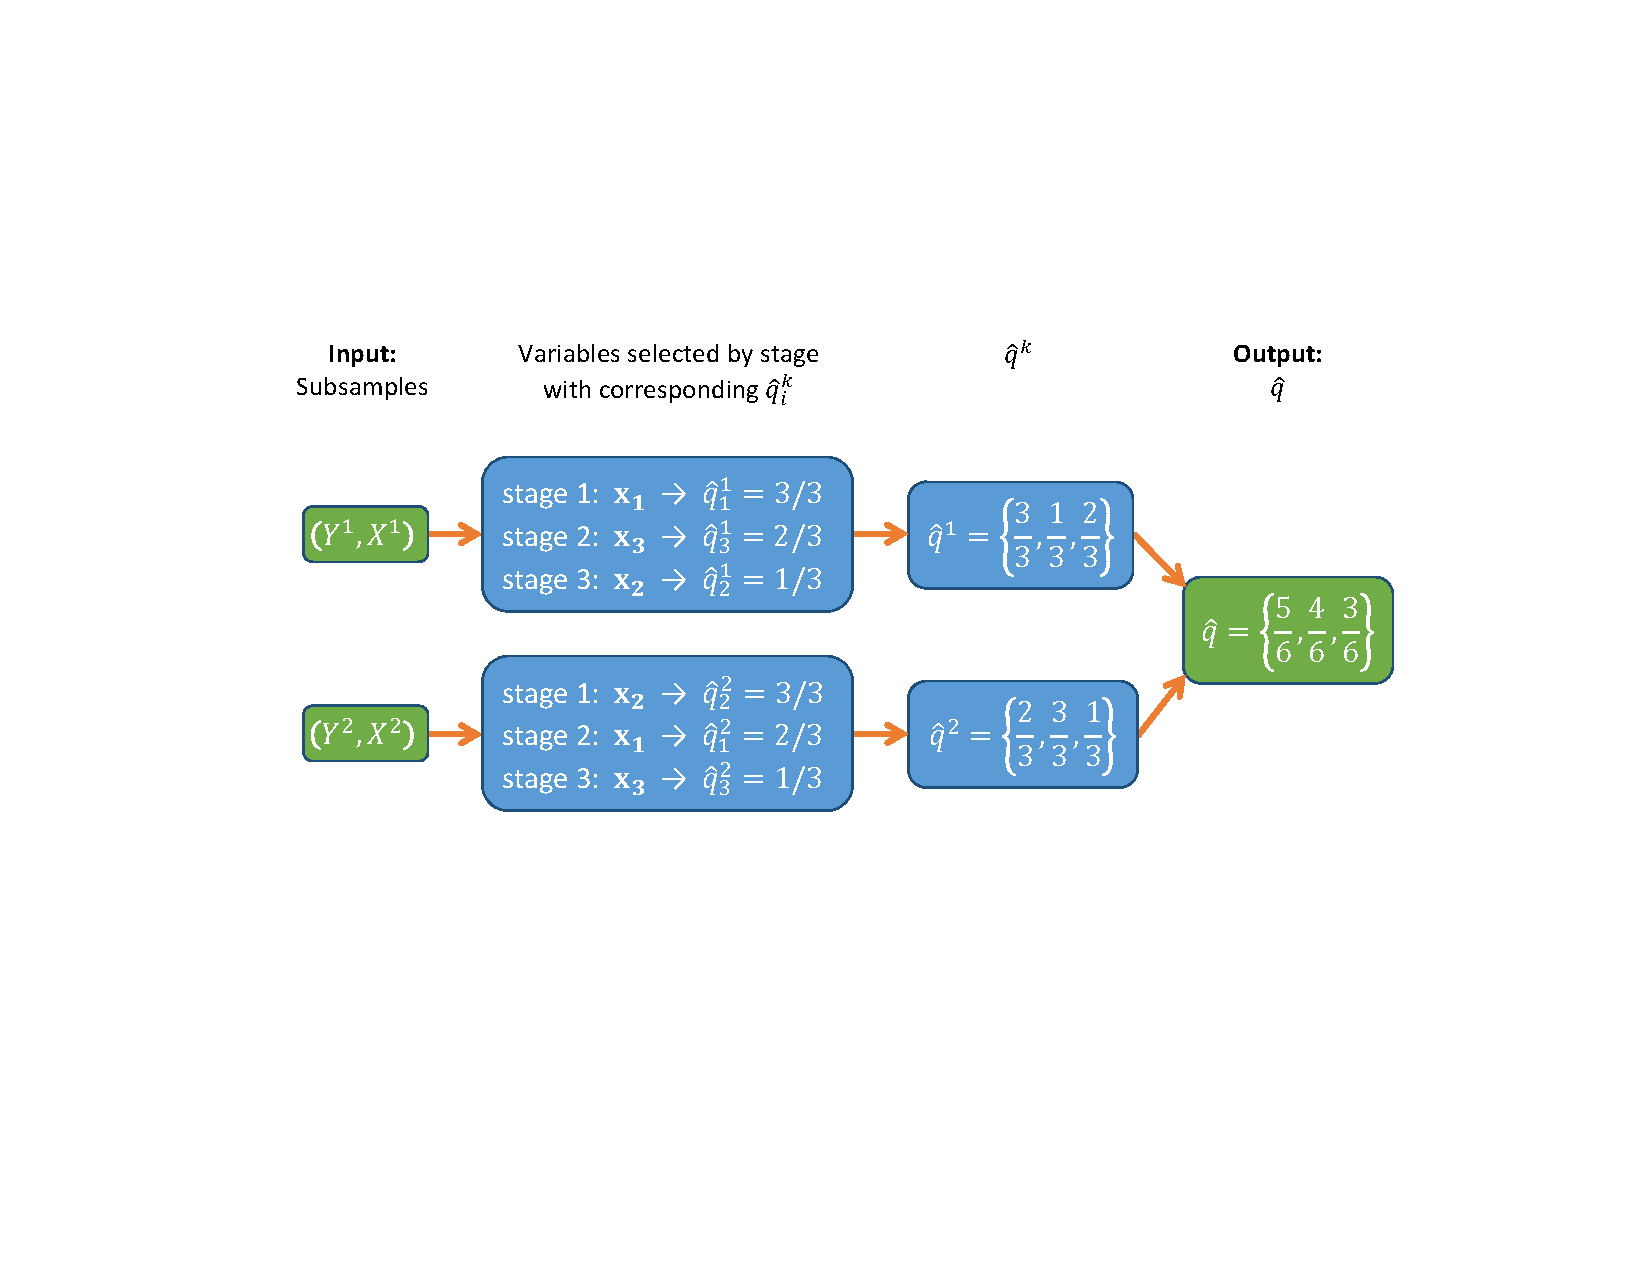
\includegraphics[width=0.66\paperwidth]{q_demo_1new.pdf}
%
  \caption{Computation of $\widehat{q}$ on 2 subsamples by least angle regression.}
%
  \label{fig:q_demo}
%
\end{figure}

After the subsamples are created, lines~\ref{inner_averaging_start}-\ref{inner_averaging_end} of Algorithm~\ref{algo:APE-lar} compute $\widehat{q}^k$, which summarizes the order that least angle regression includes each $\mathbf{x}_i$ across all stages (see Figure~\ref{fig:q_demo}). The unrestricted least angle regression ranks variables by the stage they enter the solution path. As shown in line~\ref{inner_averaging_end} of Algorithm~\ref{algo:APE-lar} and Figure~\ref{fig:q_demo}, variables included at earlier stages have larger $\widehat{q}^k_i$ values: the first variable included is assigned $1$, the last is assigned $1/\widetilde{p}$, while the rejected variables are assigned $0$ (which occurs only when $p > n$). Thus, the$L_0$ solution path is obtained by ranking the $\mathbf{x}_i$ according to their $\widehat{q}^k_i$ values.

\citet[Theorem 2]{zhang09} implies that, on average, variables with the largest $\widehat{q}^k_i$ values are more likely to be informative. The $\widehat{q}^k_i$ may be sensitive in high-dimensional spaces to multicollinearity, sampling randomness, and noise. In these circumstances, a redundant variable may be included at an early stage in some $\left( Y^k, X^k \right)$ subsample. Algorithm~\ref{algo:APE-lar} reduces the impact of sensitivity in the $\widehat{q}^k_i$ by computing $\widehat{q} := \frac{1}{K} \sum_{k=1}^{K} \widehat{q}^k$ and ranking the $\mathbf{x}_i$ according to $\widehat{q}_i$ (the $i$\textsuperscript{th} entry in $\widehat{q}$), to arrive at the average $L_0$ solution path. The average $L_0$ solution path is formally defined as follows.

%%%%%%%%%%%%%%%%%%%%%%%%%%%%%%%%%%%%%%%%%%%%%%%%%%%%%%%%%%%%%%%%%%%%%%%%%%%%%%%%%%%%%%%

\begin{definition}[average $L_0$ solution path]
  %
  Define the \textbf{average $L_0$ solution path} of least angle regression on $\left\{ \left( Y^k, X^k \right) \right\}_{k=1}^{K}$ to be the (decreasing) rank order of the $\mathbf{x}_i$ variables based on their corresponding $\widehat{q}_i$ values. For example, in Figure~\ref{fig:q_demo}, the $\widehat{q}_i$ for $\mathbf{x}_1$, $\mathbf{x}_2$ and $\mathbf{x}_3$ are, respectively, $\widehat{q}_1 = 5/6$, $\widehat{q}_2 = 4/6$ and $\widehat{q}_3 = 3/6$. Thus, the average $L_0$ solution path may be represented as an ordered set $\left\{ \left\{ \mathbf{x}_1 \right\}, \left\{ \mathbf{x}_1, \mathbf{x}_2 \right\}, \left\{ \mathbf{x}_1, \mathbf{x}_2, \mathbf{x}_3 \right\} \right\}$.
  %
  \label{def:L_0_solution_path}
  %
\end{definition}

%%%%%%%%%%%%%%%%%%%%%%%%%%%%%%%%%%%%%%%%%%%%%%%%%%%%%%%%%%%%%%%%%%%%%%%%%%%%%%%%%%%%%%%

The solar algorithm, summarized in Algorithm~\ref{algo:solar}, is presented under the generic framework of forward regression and can easily be adapted to least angle regression, forward or backward selection algorithms. Using the \citet{zhang09} framework, we prove solar variable selection consistency and variable ranking accuracy on the average $L_0$ path (see Appendix~A).

%%%%%%%%%%%%%%%%%%%%%%%%%%%%%%%%%%%%%%%%%%%%%%%%%%%%%%%%%%%%%%%%%%%%%%%%%%%%%%%%%%%%%%%

\begin{algorithm}[ht]

  \SetKwData{Left}{left}\SetKwData{This}{this}\SetKwData{Up}{up}
  \SetKwFunction{Union}{Union}\SetKwFunction{FindCompress}{FindCompress}
  \SetKwInOut{Input}{input}\SetKwInOut{Output}{output}

  \smallskip
  Randomly select 20\% of the sample points as the validation set; denote the remaining points as the training set\;

  Estimate $\widehat{q}$ using Algorithm~\ref{algo:APE-lar} on the training set and compute $Q(c) = \left\{ \mathbf{x}_j \; \vert \; \widehat{q}_j \geqslant c, \forall j\right\}$ for all $c \in \left\{ 1, 0.98, \ldots, 0.02, 0 \right\}.$

  Run an OLS regression of each $Q(c)$ on $Y$ using the training set and find $c^*$, the value of $c$ that minimizes the validation error\;

  Compute the OLS coefficients of $Q(c^*)$ on $Y$ using the whole sample.

  \caption{Subsample-ordered least-angle regression (solar) \label{algo:solar}}
\end{algorithm}

%%%%%%%%%%%%%%%%%%%%%%%%%%%%%%%%%%%%%%%%%%%%%%%%%%%%%%%%%%%%%%%%%%%%%%%%%%%%%%%%%%%%%%%

In Algorithm~\ref{algo:solar}, variables are included into forward regression according to their rank order in the average $L_0$ solution path, represented by $\left\{ Q(c) \vert c = 1, 0.98, \ldots, 0\right\}$ in Algorithm~\ref{algo:solar}. We use $\widehat{q}$ from Algorithm~\ref{algo:APE-lar} to generate a list of variables $Q \left( c \right) = \left\{ \mathbf{x}_j \; \vert \; \widehat{q}_j \geqslant c, \forall j \leqslant p \right\}$. For any $c_1 > c_2$, $Q\left(c_1\right) \subset Q\left(c_2\right)$, implying a sequence of nested sets $\left\{ Q(c) \vert c = 1, 0.98, \ldots, 0\right\}$. Each $c$ denotes a stage of forward regression. For a given value of $c$, $Q(c)$ denotes the set of variables with $\left\Vert \beta_i \right\Vert_0=1$ on average and $Q(c) - Q(c - 0.02)$ is the set of variables with $\left\Vert \beta_i \right\Vert_0$ just turning to $1$ at $c$. Therefore, $\left\{ Q(c) \vert c = 1, 0.98, \ldots, 0\right\}$ is the average $L_0$ solution path of Definition~\ref{def:L_0_solution_path}. Variables that are more likely to be informative have larger $c$ values in $Q(c)$ and will be selected first by the solar algorithm.

\subsection{Solar optimized by coordinate descent}

The solar algorithm can easily be generalized to use coordinate descent. For lasso, least angle regression or coordinate descent generates a solution path parameterized by the $\beta_i$ and the shrinkage parameter $\lambda$. Thus, to reprogram solar to use coordinate descent, we simply replace Algorithm~\ref{algo:APE-lar} with Algorithm~\ref{algo:APE-cd}, which records the order of variable selection along the coordinate descent solution path.

\smallskip
\begin{algorithm}[ht]

  \SetKwData{Left}{left}\SetKwData{This}{this}\SetKwData{Up}{up}
  \SetKwFunction{Union}{Union}\SetKwFunction{FindCompress}{FindCompress}
  \SetKwInOut{Input}{input}\SetKwInOut{Output}{output}

  \smallskip
  \Input{$\left( Y, X \right)$.}

  generate $K$ subsamples $\left\{ \left( Y^k, X^k \right) \right\}^{K}_{k=1}$ by randomly remove $1/K$ of observations in $\left( Y, X \right)$\;

  set $\widetilde{p} = \min\left\{ n_{\mathrm{sub}}, p \right\}$ \;

  \For{ k := 1 to K, stepsize = 1 \nllabel{outer_averaging_start3} }{

    denote $\lambda_s$ as the shrinkage parameter value that coordinate descent lasso selects $s$ variables, $\forall s \in \left[ 0, \widetilde{p}\right]$;

    run a pathwise coordinate descent for lasso on $\left( Y^k, X^k \right)$, $\forall \lambda \in \left\{\lambda_0, \lambda_1, \ldots, \lambda_{\widetilde{p}},\right\}$

    record the order of variable inclusion at each $\lambda \in \left\{\lambda_0, \lambda_1, \ldots, \lambda_{\widetilde{p}},\right\}$\;

    define $\widehat{q}^k = \mathbf{0} \in \mathbb{R}^p$\;

    $\forall i,s \in \mathbf{N}^+$, if $\mathbf{x}_i$ is included at $\lambda = \lambda_s$ and excluded at $\lambda_{s-1}$, set $\widehat{q}^k_i= (\widetilde{p} + 1 - s) / \widetilde{p}$, where $\widehat{q}^k_i$ is the $i$\textsuperscript{th} entry of $\widehat{q}^k$\;

  }

  $\widehat{q} := \frac{1}{K} \sum_{k=1}^{K} \widehat{q}^k$\; \nllabel{outer_averaging_end3}

  \Return $\widehat{q}$

\caption{average $L_0$ solution path estimation via coordinate descent \label{algo:APE-cd}}

\end{algorithm}

\begin{figure}[ht]
  %
  \centering
  %
  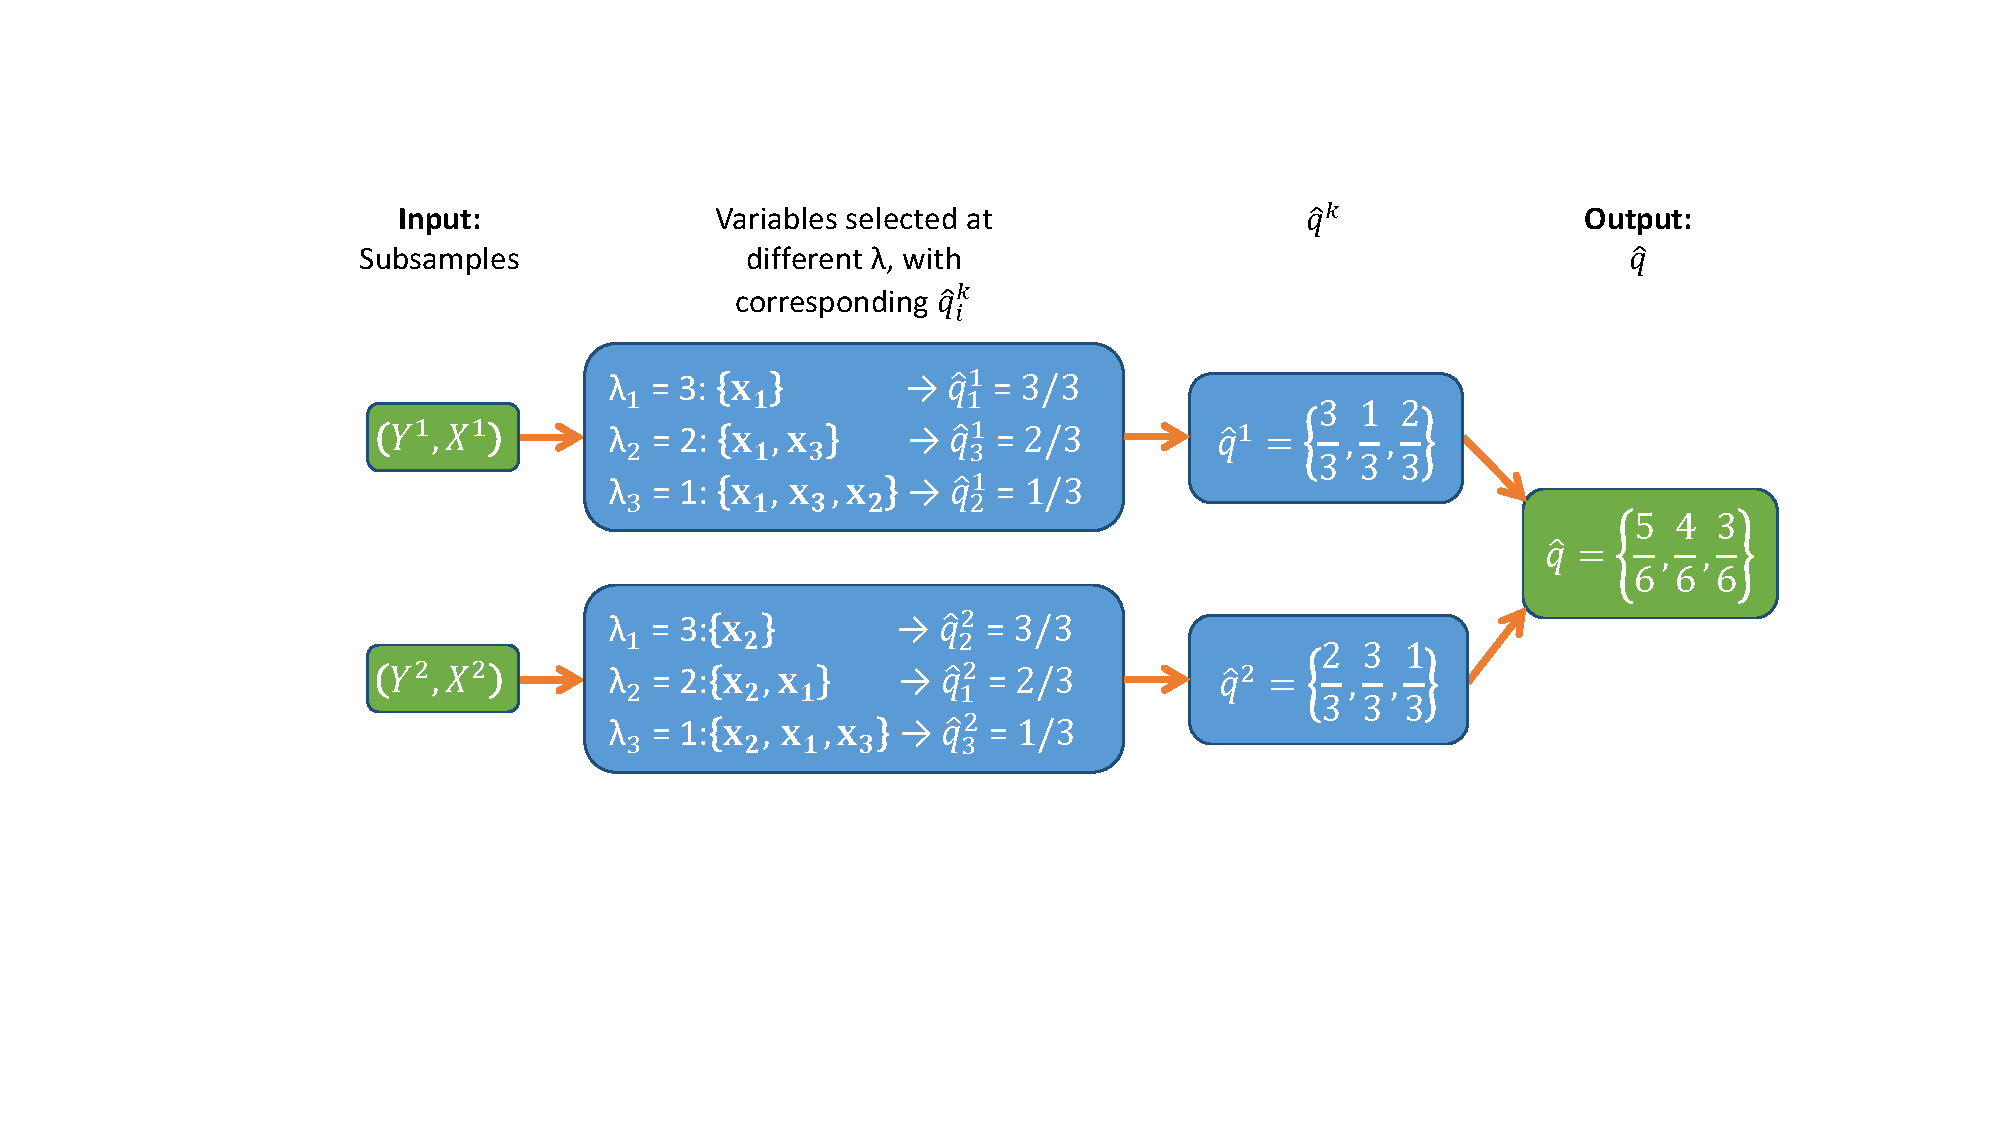
\includegraphics[width=0.66\paperwidth]{q_demo_3.pdf}
  %
  \caption{Computation of $\widehat{q}$ on 2 subsamples using coordinate descent.}
  %
  \label{fig:q_demo_3}
  %
\end{figure}

Algorithm~\ref{algo:APE-cd} serves the same purpose as Algorithm~\ref{algo:APE-lar}: to estimate the average $L_0$ path. Algorithm~\ref{algo:APE-cd} uses $\lambda$ to record the order that each variable enters the path. Consider the example in Figure~\ref{fig:q_demo_3}. To re-parameterize the solution path, we denote $\lambda_s$ to be the $\lambda$ value that coordinate descent lasso includes $s$ variables, $\forall s\in \left( 0, \min \left\{ n/2, p \right\} \right]$, giving a sequence of $\lambda$ for grid search. In each subsample $\left( Y^k, X^k \right)$, we train a standard pathwise coordinate descent for lasso, allowing $\lambda$ to increase stepwise within the grid $\left\{\lambda_1, \ldots, \lambda_{ \min \left\{ n/2, p \right\} } \right\}$, where $\lambda_1 \geqslant \ldots \geqslant \lambda_{ \min \left\{ n/2, p \right\} }$. In Figure~\ref{fig:q_demo_3}, when $\lambda \leqslant \lambda_3$ at subsample $\left( Y^1, X^1 \right)$, all three variables are selected in the solution path, implying that $\widehat{q}^1_i \geqslant 1/3$ for all variables. When $\lambda$ increases to $\lambda_2$, only $\{\mathbf{x}_3, \mathbf{x}_1\}$ survive the harsher shrinkage, implying that they should be ranked higher than $\mathbf{x}_2$. As a result, $\widehat{q}^1_1, \widehat{q}^1_3 \geqslant 2/3$ and $\widehat{q}^1_2 = 1/3$. When $\lambda$ reaches $\lambda_3$, only $\{\mathbf{x}_1\}$ remains, leaving $\widehat{q}^1_1 = 3/3$ and $\widehat{q}^1_3 = 2/3$. Applying the same method to each subsample produces the same $\widehat{q}$ as Algorithm~\ref{algo:APE-lar}.

\subsection{Generalization to lasso variants}
\label{subsec:variant}

Because it is trained by least angle regression or coordinate descent, solar can easily be extended to several lasso variants:

\begin{itemize}
  %
  \item `Grouped solar' is invoked by forcing specific variables to be simultaneously selected into the solution path;
  %
  \item `Adaptive solar' is obtained by weighting variable rankings in the average $L_0$ path according to their OLS coefficients;
  %
  \item `Solar elastic net' or `fused solar' is derived by replacing the coordinate descent loss function in Algorithm~\ref{algo:APE-cd} with the $L_1$-$L_2$ loss
    %
    \begin{equation}
      %
      \left\Vert Y -X\beta \right\Vert_2^2 + \lambda^{(1)} \left\Vert \beta \right\Vert_1 + \lambda^{(2)} \left\Vert \beta \right\Vert_2^2
      %
    \end{equation}
    %
    or fused loss
    %
    \begin{equation}
      %
      \left\Vert Y -X\beta \right\Vert_2^2 + \lambda^{(1)} \left\Vert \beta \right\Vert_1 + \lambda^{(2)} \sum_{j=2}^{p} \left\vert \beta_j - \beta_{j-1} \right\vert_1.
      %
    \end{equation}
    %
\end{itemize}

Furthermore, many lasso enhancements (e.g., safe/strong rules, post-lasso hypothesis testing) may be applied to solar because they use the same optimization methods. Rather than competing with the lasso enhancements, solar supplements them by improving variable selection performance and computation speed in large-scale applications.

\section{Solar advantages over lasso variants, lasso rules, and variable screening \label{section:adv}}

In this section, we use a series of examples to demonstrate the advantages of the solar algorithm for post-selection hypothesis testing, in the presence of complicated dependence structures, and in terms of its robustness to the \emph{irrepresentable condition} (IRC).

\subsection{Post-selection hypothesis testing}

A major advantage of solar is its amenability to post-selection testing. Because the lasso tests \citep{lockhartall14, taylor2014exact} are based on forward regression, they may be adapted to solar. More interestingly, it is straightforward to adapt the data-splitting tests \citep{wasserman2009high,meinshausen2009p} to solar. We illustrate this point using Example~1.

\smallskip
\noindent
\textbf{Example 1.} Consider the DGP
%
\begin{equation}
  Y = \mathbf{x}_0 + 2 \mathbf{x}_1 + 3 \mathbf{x}_2 + 4 \mathbf{x}_3 + 5 \mathbf{x}_4 + \sum_{j=5}^{p} 0 \cdot \mathbf{x}_j + e,
\end{equation}
%
where $\mathbf{x}_i$, $i=0,\dots,p$, are standard Gaussian variables with pairwise correlations of $0.5$, $e$ is a standard Gaussian noise term, and $p/n=100/100$.

Following \citet[Example~4.1]{romano2019multiple} and \citet{diciccio2020exact}, we conduct data-splitting tests by randomly separating the data into two portions of 50 observations. In the first round, one portion is used for solar or lasso selection and the other for testing. In the second round, the roles of the two portions are reversed. As a result, the p-values of any given variable are uncorrelated across the two rounds. Thus, we may apply Theorem~3.2 of \citet{romano2019multiple} and compute the average p-value across the two rounds to conduct a valid t-test for any selected covariate.

\citet{diciccio2020exact} stresses the importance of retaining residual degrees of freedom to ensure accurate tests. Because solar yields sparse and accurate variable selection (Section~\ref{section:comp}), it conserves residual degrees of freedom, improving the reliability of post-selection p-values. Figure~\ref{fig:p_value_compare} plots the average p-values for the informative variables $\{\mathbf{x}_0,\ldots,\mathbf{x}_4\}$ from post-solar and post-lasso data-splitting tests using 100 repetitions. While the solar and lasso p-values are less than $0.05$ for the stronger signals $\{\mathbf{x}_1,\ldots,\mathbf{x}_4\}$, more than $25\%$ of the lasso p-values exceed $0.05$ for the weakest signal $\mathbf{x}_0$, implying non-trivial false non-rejection of $H_0$. By contrast, the solar p-value boxplot is very compact for $\mathbf{x}_0$, with only $5$ out of $100$ above $0.05$. Hence, solar p-values are more reliable for detecting weak signals with small $n$ and large $p$.

\begin{figure}[ht]
%
  \centering
%
  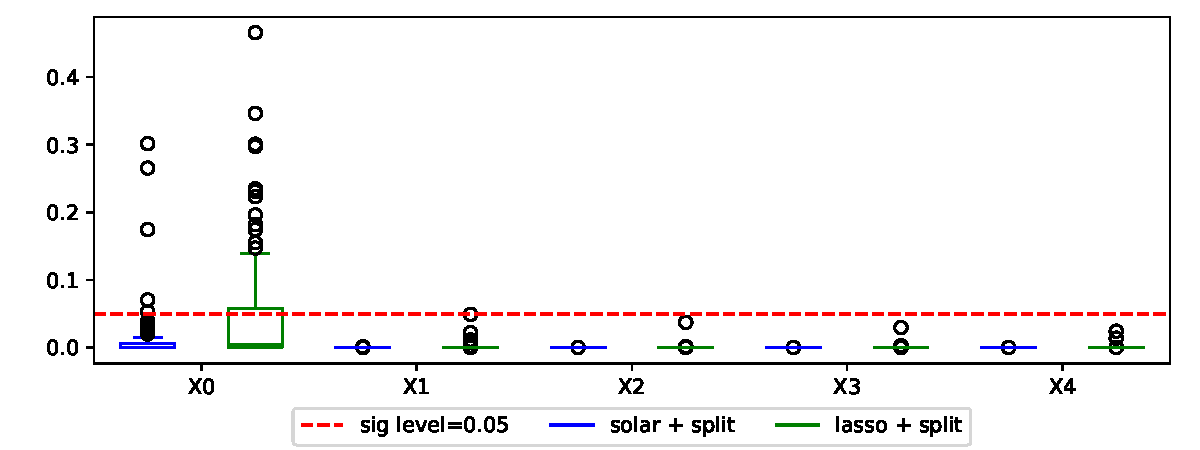
\includegraphics[width=0.7\paperwidth]{p_value_compare.pdf}
%
  \caption{Average p-value boxplots for data-splitting t-tests with solar and lasso.}
%
  \label{fig:p_value_compare}
%
\end{figure}

Moreover, the solar $L_0$ path may also assist with the formulation of $H_0$ for $p>n$. Because conserving residual degrees of freedom is so important, tests on the selection (omission) of redundant (informative) variables trigger decisions on which $\beta_i$ to test. \citet[Theorem~2]{zhang09} shows that the earlier a variable enters the $L_0$ path, the more likely it is informative, implying that variables should be tested in rank order. Given the solar ranking is more robust than lasso to settings of the irrepresentable condition, sampling noise, multicollinearity, and other issues, it is likely to provide more reliable guidance on the order to test the $\beta_i$. $\blacksquare$


\subsection{Complicated dependence structures\label{section:example}}

Another advantage of solar is that the average $L_0$ solution path is more robust to outliers, multicollinearity, and noise in high-dimensional spaces. Thus, solar is likely to be more reliable than other variable selection methods under complicated dependence structures. We illustrate the point with the following two (Bayesian network) examples.

\begin{figure}[ht]
%
  \centering
  %
  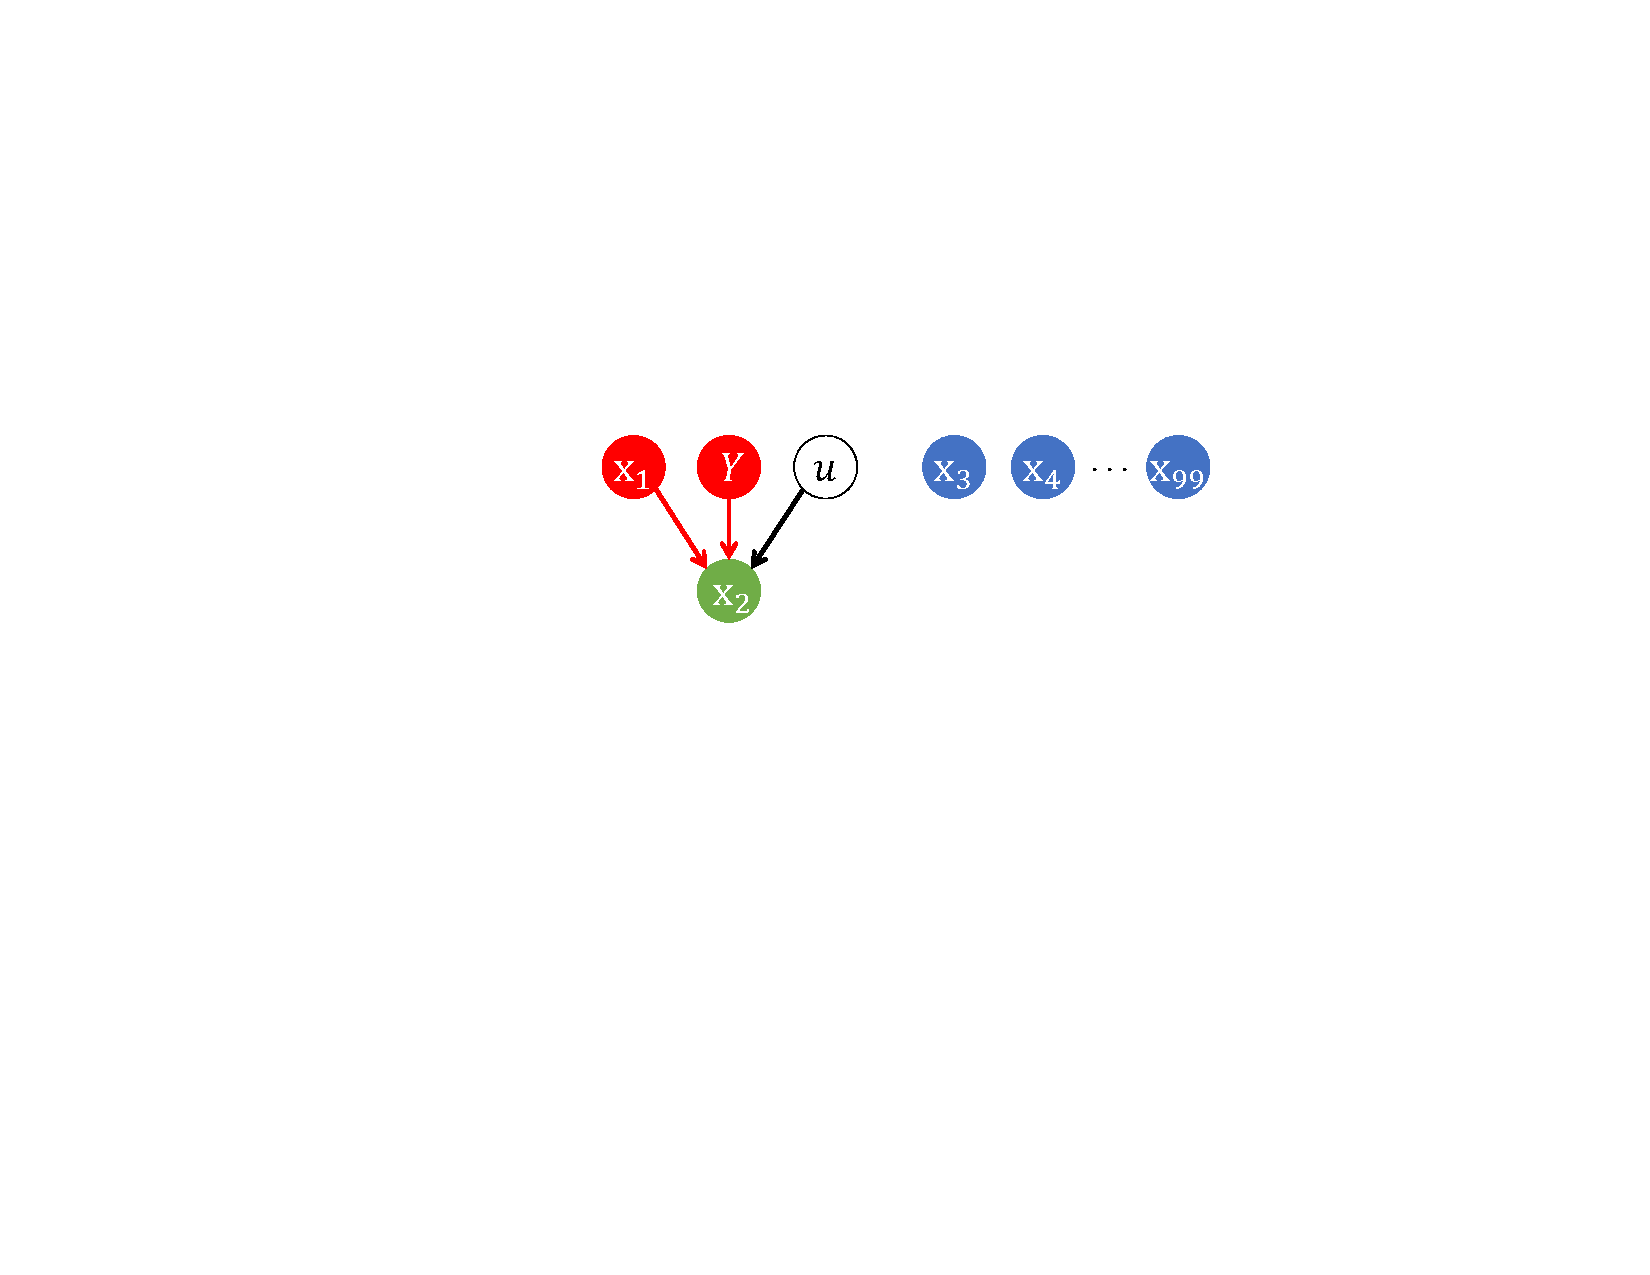
\includegraphics[width=0.35\paperwidth]{uncond_example.pdf}
  %
  \caption{Y is unconditionally uncorrelated with an informative $\mathbf{x}_1$.}
  %
  \label{fig:uncond_example}
%
\end{figure}

The first example is a common empirical regression problem: \emph{informative variables} that are \emph{unconditionally uncorrelated to} $Y$ in the DGP. In Figure~\ref{fig:uncond_example}, $\mathbf{x}_1$ and $\mathbf{x}_2$ are informative for $Y$, while $\mathbf{x}_1$ and $Y$ are independent. For example, in biostatistics, concussion ($\mathbf{x}_1$) or a brain tumor ($Y$) may cause headaches ($\mathbf{x}_2$), implying that concussion history is when attempting to diagnose a brain tumor. In this setting, Example~2a shows that solar is more reliable than post-lasso rules and variable screening.

\smallskip
\noindent
\textbf{Example 2a.} In Figure~\ref{fig:uncond_example}, there are $100$ variables and $\mathbf{x}_2$ is (causally) generated by its parents $\left\{ \mathbf{x}_1, Y \right\}$ as follows,
%
\begin{equation}
  %
  \mathbf{x}_2 = \alpha_1 \mathbf{x}_1 + \alpha_2 Y + u,
  %
  \label{eqn:collider_1}
  %
\end{equation}
%
where $\mathbf{x}_1$ is unconditionally uncorrelated with $Y$, $\mathbf{x}_1$ and $Y$ are both unconditionally and conditionally uncorrelated with the redundant variables $\{\mathbf{x}_3, \ldots, \mathbf{x}_{99}\}$, $\left\{\alpha_1, \alpha_2 \right\}$ are population regression coefficients, and $u$ is a Gaussian noise term. If $Y$ is chosen to be the response variable, the population regression equation is
%
\begin{equation}
  %
  Y = -\frac{\alpha_1}{\alpha_2} \mathbf{x}_1 + \frac{1}{\alpha_2} \mathbf{x}_2 - \frac{1}{\alpha_2}u.
  %
  \label{eqn:collider_2}
  %
\end{equation}
%
Note that $\mathbf{x}_1$ and $\mathbf{x}_2$ are both informative variables for $Y$. However, since $\mathbf{x}_1$ is unconditionally uncorrelated with $Y$ in the population, some post-lasso rules [such as the strong rule \citep{tibshirani2012strong} and the safe rule \citep{ghaoui2010safe}] may be prone to rejecting $\mathbf{x}_1$. For a given value of the shrinkage parameter $\lambda$ in grid search, the base strong rule and the safe rule for lasso to reject a selected variable, respectively, satisfies (\ref{eqn:safe_rule}) and (\ref{eqn:strong_rule}):
%
\begin{eqnarray}
  %
  \left\vert \mathbf{x}_i^T Y \right\vert < & \lambda - \left\Vert \mathbf{x}_i \right\Vert_2 \left\Vert Y \right\Vert_2 \frac{\lambda_{max} - \lambda} {\lambda_{max}} ; \label{eqn:safe_rule} \\
  %
  \left\vert \mathbf{x}_i^T Y \right\vert < & 2\lambda - \lambda_{max} , \label{eqn:strong_rule}
  %
  \label{eqn:post_estmation_rule}
  %
\end{eqnarray}
%
where the $\mathbf{x}_i$ are standardized and $\lambda_{max}$ is the value of the shrinkage parameter that rejects all the variables. Both rules are based on the unconditional covariance between $\mathbf{x}_i$ and $Y$. For a given value of $\lambda$ (typically selected by CV), lasso will likely select $\mathbf{x}_1$ and $\mathbf{x}_2$ along with redundant variables from $\left\{ \mathbf{x}_3, \ldots, \mathbf{x}_{99} \right\}$ [because the DGP does not violate the IRC]. Since $\mathrm{corr} \left( \mathbf{x}_1, Y \right) = \mathrm{corr} \left( \mathbf{x}_3, Y \right) =  \cdots = \mathrm{corr} \left( \mathbf{x}_{99}, Y \right) = 0$ in the population, the sample value of $\left\vert \mathbf{x}_1^T Y \right\vert$ will be approximately as small as the $\left\vert \mathbf{x}_i^T Y \right\vert$ of any redundant variable. Put another way, $\mathbf{x}_1$ cannot be distinguished from the redundant variables by the value of $\left\vert \mathbf{x}_i^T Y \right\vert$. To ensure $\mathbf{x}_1$ is not rejected by (\ref{eqn:safe_rule}) or (\ref{eqn:strong_rule}), both $\lambda - \left\Vert \mathbf{x}_1 \right\Vert_2 \left\Vert Y \right\Vert_2 \frac{\lambda_{max} - \lambda} {\lambda_{max}}$ and $2\lambda - \lambda_{max}$ must be smaller than $\left\vert \mathbf{x}_1^T Y \right\vert$. However, this will lead to two problems. First, decreasing the right-hand side of (\ref{eqn:safe_rule}) and (\ref{eqn:strong_rule}) will reduce the value of $\lambda$, implying that lasso will select more redundant variables. Second, since $\left\vert \mathbf{x}_1^T Y \right\vert$ will be approximately as small as the $\left\vert \mathbf{x}_i^T Y \right\vert$ of any redundant variable selected by lasso, not rejecting $\mathbf{x}_1$ (by reducing both right-hand side terms) may result in (\ref{eqn:safe_rule}) and (\ref{eqn:strong_rule}) retaining redundant variables.

Variable screening methods \citep{fan2008sure} may also be prone to selecting redundant variables. Screening ranks variables decreasingly based on the absolute values of their unconditional correlations to $Y$, selecting the top $w$ variables (with $w$ selected by CV, bootstrap, or BIC). Since $\mathrm{corr} \left( \mathbf{x}_2, Y \right) \neq 0$ in the population, screening will rank $\mathbf{x}_2$ highly. However, it may not rank $\mathbf{x}_1$ highly because $\mathrm{corr} \left( \mathbf{x}_1, Y \right) = 0$ in the population. Thus, some redundant variables may be ranked between $\mathbf{x}_2$ and $\mathbf{x}_1$, implying that if both $\mathbf{x}_1$ and $\mathbf{x}_2$ are selected, screening will select redundant variables.

The average $L_0$ solution path will not suffer the same problems. For convenience, assume $-\alpha_1 / \alpha_2 > 0$ and $p/n = 100/200$ or smaller. For least angle regression, as $\left\Vert \beta_2 \right\Vert_1$ increases at stage~1 (i.e., as $\mathbf{x}_2$ is `partialled out' of $Y$), the unconditional correlation between $Y - \beta_2 \mathbf{x}_2$ and $\mathbf{x}_1$ will increase above $0$ significantly while the marginal correlation between $Y - \beta_2 \mathbf{x}_2$ and any redundant variable will remain approximately $0$. Thus, in the $L_0$ solution path and, hence, the average $L_0$ solution path, $\mathbf{x}_1$ will be included immediately after $\mathbf{x}_2$ is included. $\blacksquare$

\citet{fan2008sure} and \citet{barut2016conditional} propose two solutions for the problems with variable screening in situations like Example~2a. However,

\begin{itemize}
  %
  \item the first approach \citep[Section~2.2 and~3]{barut2016conditional} assumes the identity of $\mathbf{x}_2$ is known, which is unlikely to be realistic in practical applications. [In Bayesian networks or probabilistic graph modelling, $\mathbf{x}_2$ is known as a \emph{collider}; \citet{barut2016conditional} refer to $\mathbf{x}_2$ as a \emph{hidden signature} variable and denote it by $X_c$];
  %
  \item the second approach \citep[Section~1 and~2.2]{barut2016conditional} suggests randomly trying out several variables to be colliders. The logic is straightforward: randomly trying out a wrong variable (like $\mathbf{x}_2$) to be a collider is harmless because conditioning on that variable will not make $corr(Y,\mathbf{x}_1) \neq 0$, nor will it cause the selection of a redundant variable. Moreover, by repeatedly randomly trying out variables, there is a non-zero probability the correct collider will eventually be uncovered, producing a statistically significant $corr(Y,\mathbf{x}_1) \neq 0$. However, using multiple trials may be inefficient and computationally expensive, especially with high-dimensional data. To improve high-dimensional efficiency, \citet{barut2016conditional} suggests trying out several variables simultaneously. However, if $corr(Y, \mathbf{x}_1) \neq 0$ were discovered after trying out, say, $\left\{\mathbf{x}_2,\mbox{other variables}\right\}$, it would still be necessary to decide which of $\left\{\mathbf{x}_2,\mbox{other variables}\right\}$ are redundant, meaning variable selection is not completed.
  %
\end{itemize}

\medskip

The second example illustrates another common problem in empirical regression: \emph{redundant variables} that are \emph{unconditionally correlated to} $Y$ in the DGP. In Figure~\ref{fig:cond_example}, the problem occurs because $\mathbf{x}_3$ and $Y$ are determined by common variables. For example, house rent ($Y$) and food expenditure ($\mathbf{x}_3$) are both determined by income ($\mathbf{x}_1$) and saving ($\mathbf{x}_2$), yet $\mathbf{x}_3$ is redundant if $\mathbf{x}_1$ and $\mathbf{x}_2$ are used to predict $Y$. In this setting, Example~2b illustrates that the strong rule, base rule, and variable screening methods may struggle to reject the redundant $\mathbf{x}_3$ even when IRC is satisfied. By contrast, solar will be less prone to selecting redundant variables.

\begin{figure}[ht]
  %
    \centering
    %
    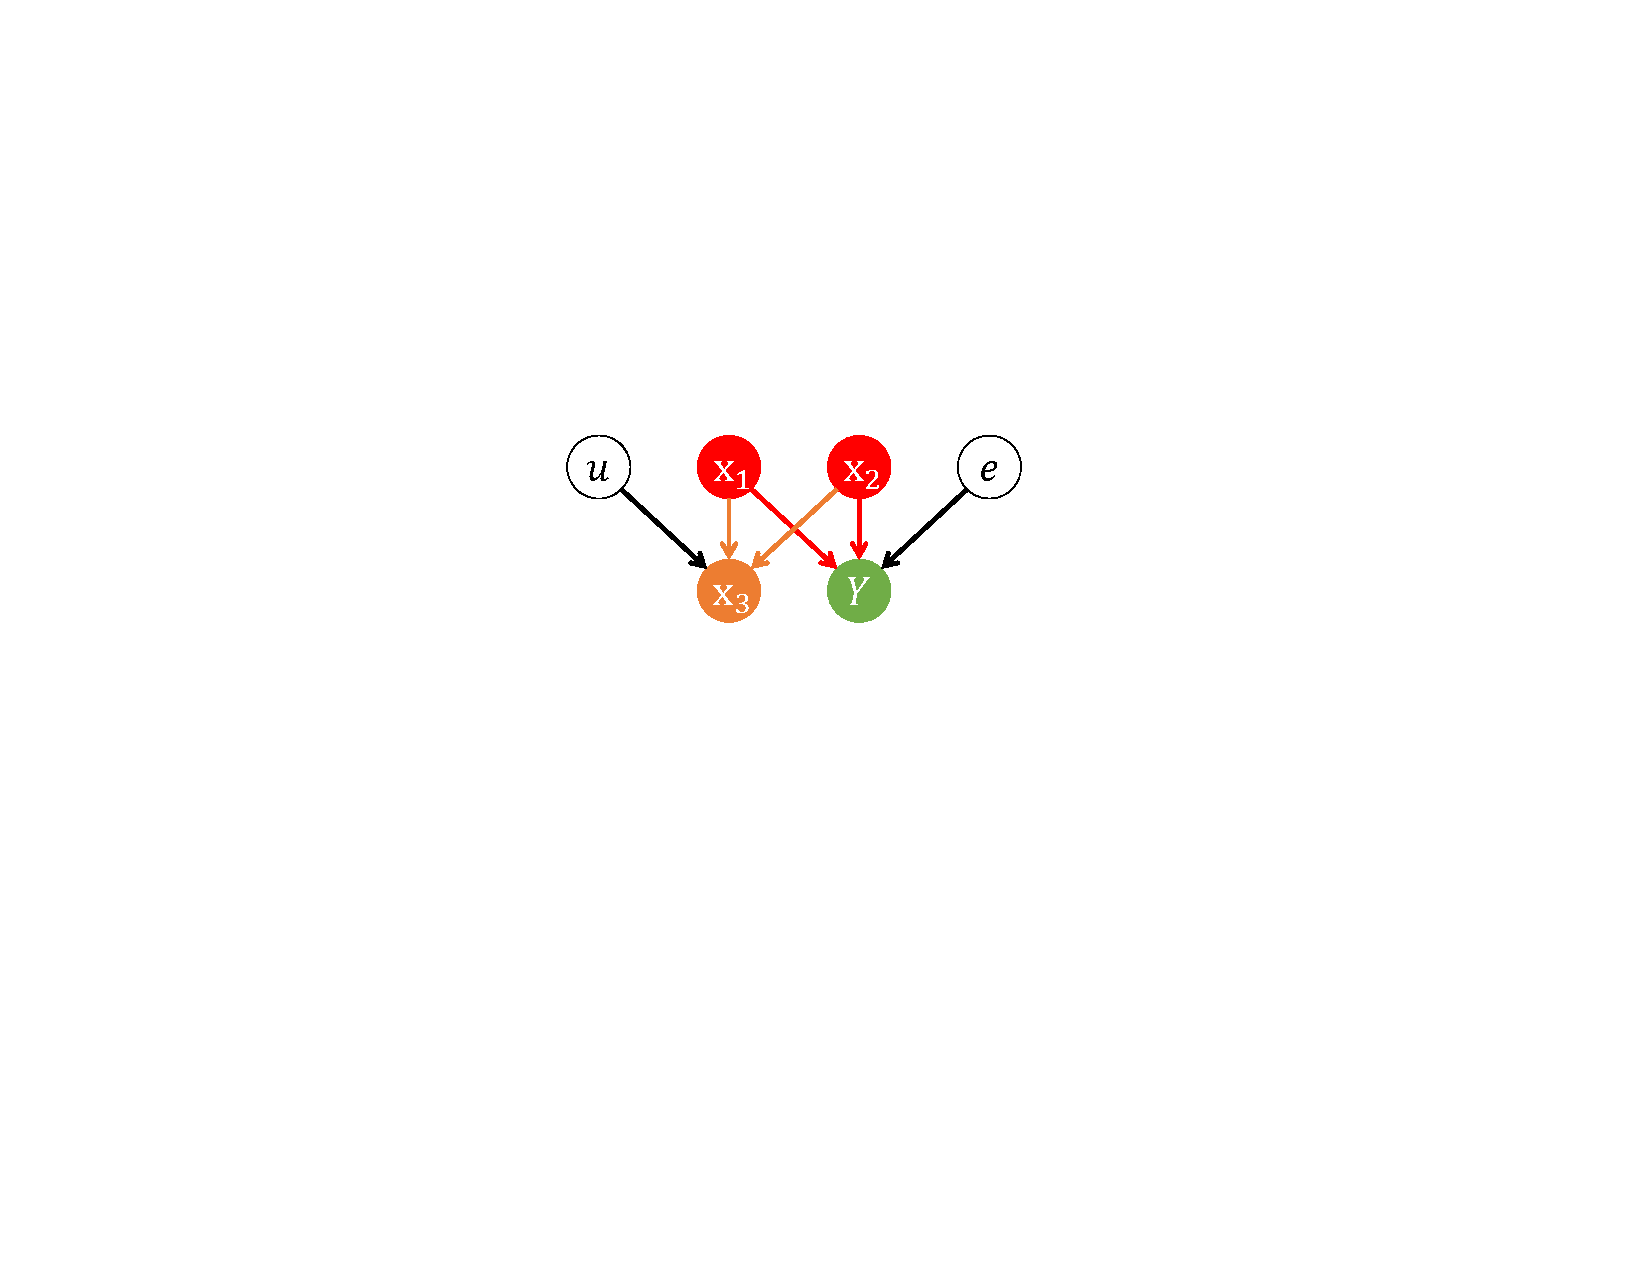
\includegraphics[width=0.35\paperwidth]{example3.pdf}
    %
    \caption{$Y$ is unconditionally correlated with a redundant $\mathbf{x}_3$.}
    %
    \label{fig:cond_example}
  %
  \end{figure}

\smallskip
\noindent
\textbf{Example 2b.} Figure~\ref{fig:cond_example} depicts the following confounding structure,
%
\begin{equation}
	%
	\begin{cases}
	%
    \mathbf{x}_3 = \frac{1}{3} \mathbf{x}_1 + \frac{1}{3} \mathbf{x}_2 + \frac{\sqrt{7}}{3} u, \\
    %
    Y = \frac{7}{10} \mathbf{x}_1 +  \frac{2}{10} \mathbf{x}_2 +  \frac{\sqrt{47}}{10} e, \\
    %
	\end{cases}
	%
	\label{eqn:example_4}
	%
\end{equation}
%
where $\mathbf{x}_1$ and $\mathbf{x}_2$ cause both $Y$ and $\mathbf{x}_3$, implying that $\mathbf{x}_3$ is unconditionally correlated to $Y$; $\mathbf{x}_1$, $\mathbf{x}_2$, $u$ and $e$ are independent; $\mathbf{x}_3$ is independent from $e$; $Y$ is independent from $u$; and all variables are standardized.

For large $n$, when the sample correlations are close to their population values, the sample marginal correlations to $Y$ are:
%
\begin{equation}
  %
  \begin{aligned}
    %
    \mathrm{corr} \left( \mathbf{x}_1, Y \right)  = & \;0.7, \\
    %
    \mathrm{corr} \left( \mathbf{x}_3, Y \right)  = & \;\mathrm{corr} \left( \frac{1}{3} \mathbf{x}_1 + \frac{1}{3} \mathbf{x}_2, \frac{7}{10} \mathbf{x}_1 +  \frac{2}{10} \mathbf{x}_2 \right)
    %
    = 0.3, \\
    %
    \mathrm{corr} \left( \mathbf{x}_2, Y \right)  = & \;0.2. \\
    %
  \end{aligned}
  %
\end{equation}
%
Because $\mathbf{x}_2$ ranks below $\mathbf{x}_1$ and $\mathbf{x}_3$ in terms of marginal correlations to $Y$, the variable screening method must select all $3$ variables---including the redundant $\mathbf{x}_3$---to avoid omitting $\mathbf{x}_2$. The base strong rule and safe rule may also have difficulty rejecting $\mathbf{x}_3$. Since $\mathrm{corr} \left( \mathbf{x}_3, Y \right)>\mathrm{corr} \left( \mathbf{x}_2, Y \right)$, if lasso selects $\mathbf{x}_3$ and $\mathbf{x}_2$ and the strong (or safe) rule is used to reject $\mathbf{x}_3$, $\mathbf{x}_2$ will also be rejected.

Forward regression, solar, and lasso will not make the same error. Because (\ref{eqn:example_4}) does not violate the IRC, variable-selection consistency of forward regression, lars, and lasso is assured from the theoretical results of \citet{zhang09} and \citet{zhaoyu06}. In forward regression, $\mathbf{x}_1$ will be included  at the first stage. After controlling for $\mathbf{x}_1$, the partial correlations (for large $n$) of both $\mathbf{x}_2$ and $\mathbf{x}_3$ with $Y$ are:
%
\begin{equation}
  %
  \begin{aligned}
    %
    \mathrm{corr} \left( \mathbf{x}_2, Y \vert \mathbf{x}_1 \right)  = & \;\mathrm{corr} \left( \mathbf{x}_2, \frac{2}{10} \mathbf{x}_2 \right)
    %
    = 0.2, \\
    %
    \mathrm{corr} \left( \mathbf{x}_3, Y \vert \mathbf{x}_1 \right)  = & \;\mathrm{corr} \left( \frac{1}{3} \mathbf{x}_1 + \frac{1}{3} \mathbf{x}_2, \frac{2}{10} \mathbf{x}_2 \right)
    %
    = 0.0667. \\
    %
  \end{aligned}
  %
\end{equation}
%
Because $\mathrm{corr}(\mathbf{x}_2, Y \vert \mathbf{x}_1)>\mathrm{corr}(\mathbf{x}_3, Y \vert \mathbf{x}_1)$, forward regression will include $\mathbf{x}_2$ not $\mathbf{x}_3$ at the second stage. After controlling for both $\mathbf{x}_1$ and $\mathbf{x}_2$, the remaining variation in $Y$ is due to $e$, which $\mathbf{x}_3$ cannot explain. Thus, CV or BIC will terminate forward regression after the second stage and $\mathbf{x}_3$ will not be selected. Similarly, because solar relies on the average $L_0$ path, it will include $\mathbf{x}_1$ and $\mathbf{x}_2$ but not $\mathbf{x}_3$. $\blacksquare$

\bigskip
Essentially, the strong rule, safe rule, and variable screening struggle in Examples~2a and~2b because they rely on unconditional correlations to $Y$, whereas informative variables in regression analysis are defined in terms of conditional correlations. In many scenarios, unconditional and conditional correlations are aligned. However, when they are not, variable selection based conditional correlation is better placed to select the informative variables.

\citet{fan2008sure} propose redeeming variable screening on $Y$ by first selecting variables with high unconditional correlations to $Y$ and then running a lasso of the residuals on the dropped variables. By contrast, solar completes variable selection in a single pass of conditional correlation ranking, reducing computational costs. Moreover, the \citet{fan2008sure} approach does not solve Example~2b type problems. At the first step, variables with high unconditional correlations to $Y$ will be selected, including the redundant $\mathbf{x}_3$. Selecting redundant variables will be more serious when $Y$ has multiple $\mathbf{x}_3$-like siblings and in complicated dependence structures where multicollinearity results in inaccurate estimates of the coefficients and standard errors in finite samples. In short, solar is likely to be more computationally efficient and better at variable selection in settings with complicated dependence structures.

%%%%%%%%%%%%%%%%%%%%%%%%%%%%%%%%%%%%%%%%%%
%%%%%%%%%%%%%%%%%%%%%%%%%%%%%%%%%%%%%%%%%%
%%%%% irrepresentable cond of solar %%%%%%
%%%%%%%%%%%%%%%%%%%%%%%%%%%%%%%%%%%%%%%%%%
%%%%%%%%%%%%%%%%%%%%%%%%%%%%%%%%%%%%%%%%%%

\subsection{Robustness to the IRC \label{subsection:irc}}

Solar is more robust to different settings of the IRC than the lasso. The IRC is considered to be sufficient and almost necessary for accurate lasso variable selection \citep{zhang09}. Here, we ignore lasso rules and variable screening since, as discussed above, their selection accuracy may be compromised by a reliance on unconditional correlations to $Y$. We define the IRC as in \citet{zhang09}.

\begin{definition}[IRC]
  Given $F \subset \left\{ 1, \ldots, p \right\}$, define $X_F$ to be the $n \times \left\vert F \right \vert$ matrix with only the full set of informative variables. Define
  %
    \begin{align}
    %
    \mu \left( F \right) = & \max \left\{ \left\Vert \left( \left( X_F \right)^T X_F \right)^{-1} \left( X_F \right)^T \mathbf{x}_j \right\Vert_1 \; \vert \; \forall j \not\in F \right\}. \notag
    %
    \end{align}
  %
  Given a constant $1 \geqslant \eta > 0$, the \emph{strong} irrepresentable condition is satisfied if $\mu \left( F \right) \leqslant 1 - \eta$ and the \emph{weak} irrepresentable condition is satisfied if $\mu \left( F \right) < 1$.$\blacksquare$
\end{definition}

\smallskip
\noindent
\textbf{Example 3.} Modify the DGP in Example~2b to match the \citet{zhaoyu06} simulations. Thus, $n = 200$, $p = 50$, and $\{\mathbf{x}_0, \ldots, \mathbf{x}_4, \mathbf{x}_6, \ldots, \mathbf{x}_{50}\}$ are generated from a zero-mean, unit-variance multivariate Gaussian distribution, where all the correlation coefficients are $0.5$. The DGP of $Y$ and $\mathbf{x}_5$ is
\begin{equation}
	%
	\begin{cases}
	%
    \mathbf{x}_5 = \omega \mathbf{x}_0 + \omega \mathbf{x}_1 + \gamma\cdot \sqrt{1 - 2\omega^2} \\
    %
    Y = 2 \mathbf{x}_0 + 3\mathbf{x}_1 + 4 \mathbf{x}_2 + 5 \mathbf{x}_3 + 6 \mathbf{x}_4 + e \\
    %
	\end{cases}
	%
	\label{eqn:dgp_x5}
	%
\end{equation}
%
where $\omega \in \mathbb{R}$, while $\gamma$ and $e$ are both standard Gaussian noise terms, independent from each other and all the other variables. Compared with Example~2b, this DGP increases the challenge of accurate selection by increasing the number of redundant variables from 1 to 46, $\{\mathbf{x}_5, \ldots, \mathbf{x}_{50}\}$. This DGP also makes it straightforward to control the IRC through $\omega$, which affects the value of $\mu \left( F \right)$.

\begin{figure}
  %
  \centering
  %
  \subfloat[\label{fig:solar_ic_type-II1}$\omega = 1/4,\;\mu\left(F\right)=1/2$, lasso]
  {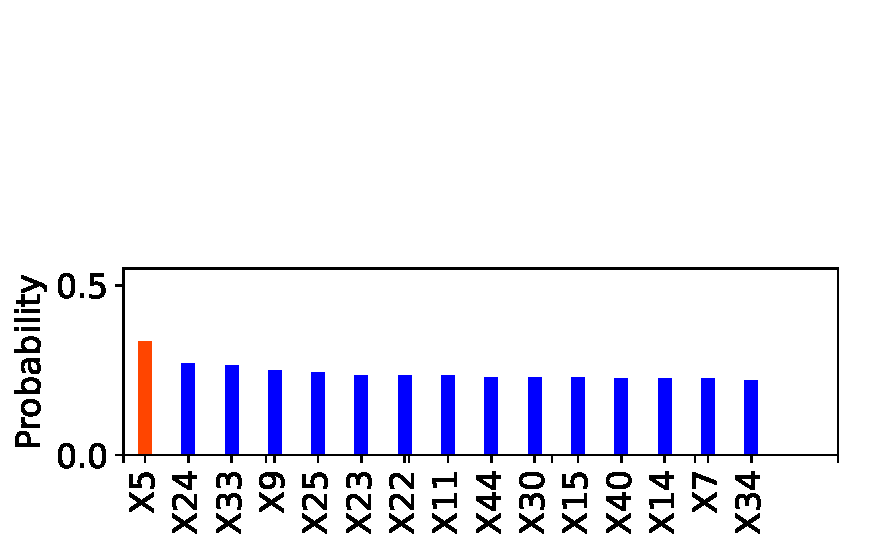
\includegraphics[width=0.25\paperwidth]{acc_plot_top20_ic_25_False_lars-crop.pdf}}
  %
  \subfloat[\label{fig:solar_ic_type-II2}$\omega = 1/3,\;\mu\left(F\right)=2/3$, lasso]
  {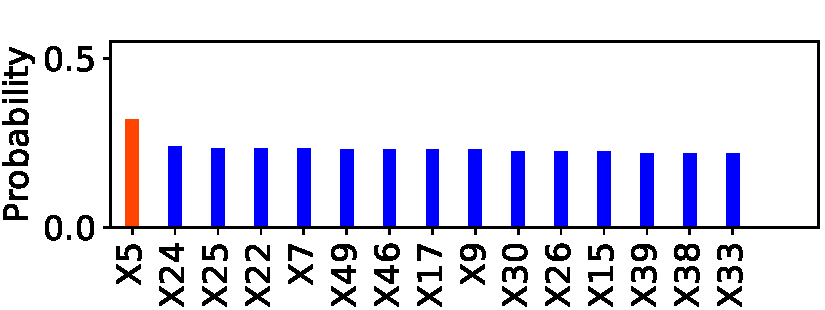
\includegraphics[width=0.25\paperwidth]{acc_plot_top20_ic_33_False_lars-crop.pdf}}
  %
  \subfloat[\label{fig:solar_ic_type-II3}$\omega = 1/2,\;\mu\left(F\right)=1$, lasso]
  {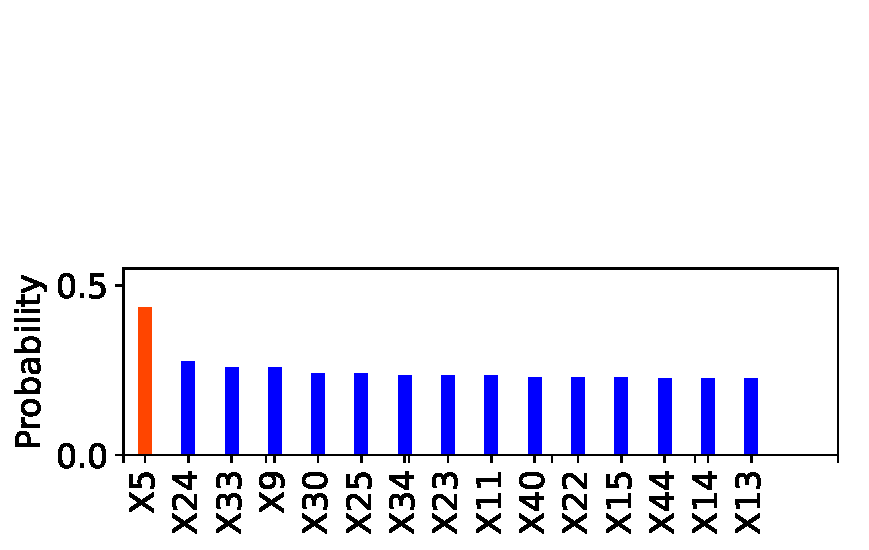
\includegraphics[width=0.25\paperwidth]{acc_plot_top20_ic_5_False_lars-crop.pdf}}

  \subfloat[\label{fig:solar_ic_type-II7}$\omega = 1/4,\;\mu\left(F\right)=1/2$, solar]
  {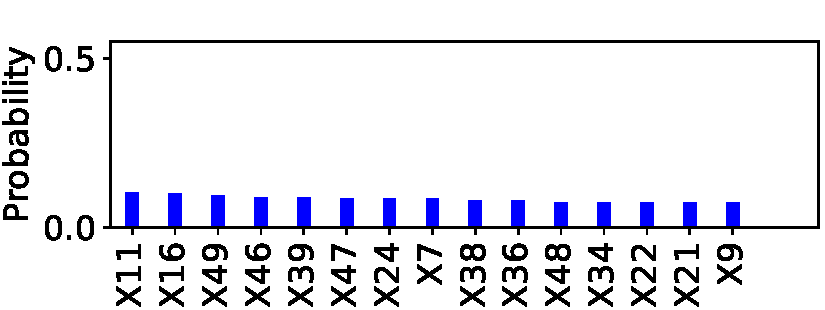
\includegraphics[width=0.25\paperwidth]{acc_plot_top20_ic_25_False_solar-crop.pdf}}
  %
  \subfloat[\label{fig:solar_ic_type-II8}$\omega = 1/3,\;\mu\left(F\right)=2/3$, solar]
  {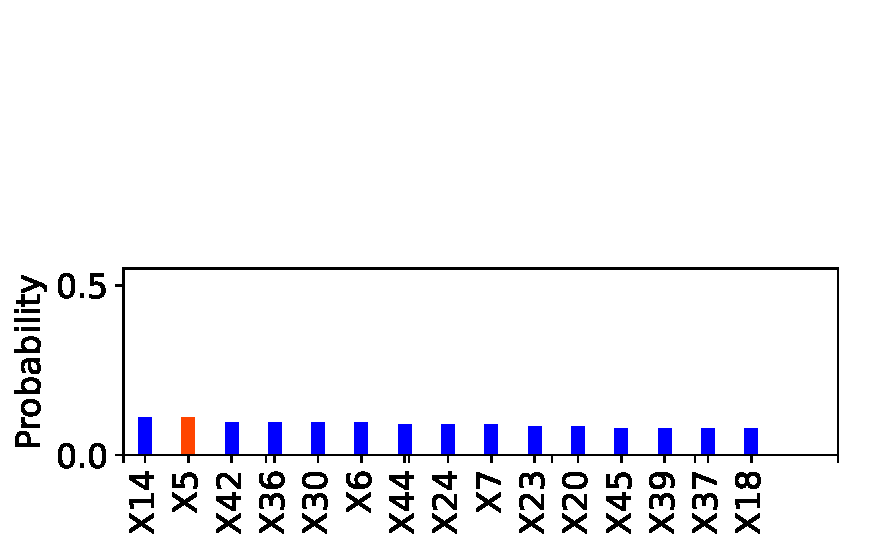
\includegraphics[width=0.25\paperwidth]{acc_plot_top20_ic_33_False_solar-crop.pdf}}
  %
  \subfloat[\label{fig:solar_ic_type-II9}$\omega = 1/2,\;\mu\left(F\right)=1$, solar]
  {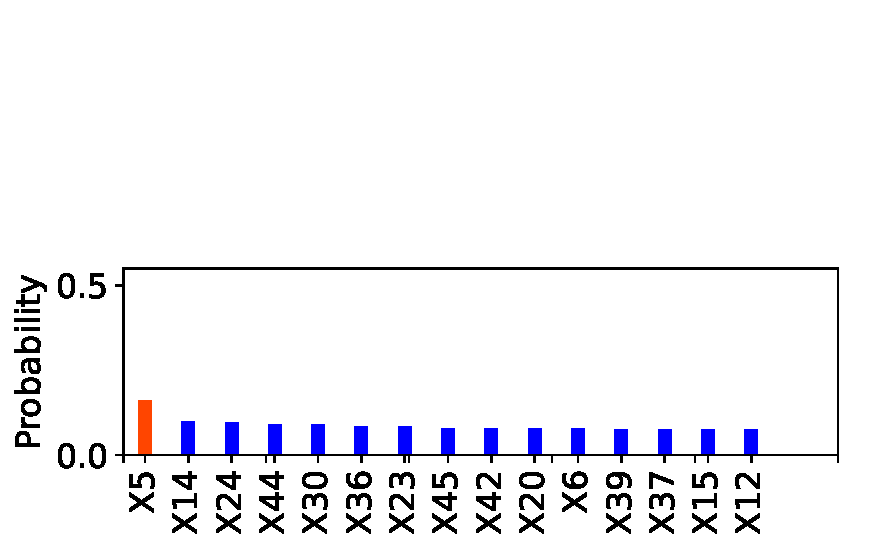
\includegraphics[width=0.25\paperwidth]{acc_plot_top20_ic_5_False_solar-crop.pdf}}
  %
  \caption{Probability of including redundant variables (top 15) in simulation~2 ($\mathbf{x}_5$ in orange).}
  \label{fig:solar_ic_type-II}
  %
\end{figure}

In (\ref{eqn:dgp_x5}), the IRC only affects the redundant $\mathbf{x}_5$. Hence, we focus on the probability of incorrectly selecting $\mathbf{x}_5$ in 200 repetitions. By setting $\omega$ to either $1/4$, $1/3$, or $1/2$, the population value of $\mu \left( F \right)$ changes, respectively, to $1/2$, $2/3$, or $1$, gradually increasing the difficulty of rejecting the redundant $\mathbf{x}_5$.

Figure~\ref{fig:solar_ic_type-II} displays the simulation results. When $\mu \left( F \right) = 1/2$, lasso wrongly includes $\mathbf{x}_5$ with probability $0.25$. By contrast, $\mathbf{x}_5$ is not among the top 15 variables selected by solar, implying a probability less than $0.1$. When $\mu \left( F \right)$ increases to $2/3$, the probability lasso includes $\mathbf{x}_5$ increases to around $0.3$. When $\mu \left( F \right)$ increases to $1$ in the population and strong IRC is violated, the probability lasso includes $\mathbf{x}_5$ rises to almost $0.5$. By contrast, the probability solar includes $\mathbf{x}_5$ is below $0.1$ even when $\mu\left(F\right)=1$. The results illustrate that solar is more robust to different settings of the IRC. $\blacksquare$


%%%%%%%%%%%%%%%%%%%%%%%
%%%%%% SECTION 4 %%%%%%
%%%%%%%%%%%%%%%%%%%%%%%

\section{Solar advantages over subsample variable selection\label{section:comp}}

In this section, we shift our focus to simulation. We demonstrate that: (i) solar offers significant improvements over lasso-type algorithms in terms of variable selection sparsity and accuracy; (ii)~replacing lasso with solar in subsample selection drastically reduces the computation load, measured by runtime. We choose the simulation settings so that, as far as possible, the comparisons are fair, representative, and generalizable. Our overall goal is to enable \emph{ceteris paribus} comparisons between solar and state-of-the-art lasso algorithms.

\subsection{Simulation competitors}

We consider a subset of lasso-type algorithms for comparison to solar. Firstly, some lasso modifications (e.g., fused lasso, grouped lasso) are designed to solve specific empirical problems that are not relevant to our paper. Secondly, it may be difficult to determine how much some variants outperform lasso.\footnote{For example, while \citet{jia2010model} show numerically that elastic net has slightly better variable-selection accuracy than lasso, they also find that ``when the lasso does not select the true model, it is more likely that the elastic net does not select the true model either'' (a point we verify in Section~\ref{section:application}). While simulations in \citet{zou2006adaptive} show that adaptive lasso outperforms lasso when $p/n<1$, it requires first computing the OLS estimates of all $\mathbf{x}_i$ coefficients, which is difficult when $p/n>1$.} Since both solar and lasso may be evaluated via least angle regression and coordinate descent, many other lasso modifications can be directly applied to solar, as discussed in Section~\ref{subsec:variant}. We do not consider information criteria for shrinkage parameter tuning. \citet{scikit-learn} points out that information criteria are over-optimistic and require a proper estimation of the degrees of freedom for the solution. Moreover, information criteria are derived asymptotically and tend to break down when the problem is badly conditioned (e.g., $p > n$).\footnote{See \url{https://scikit-learn.org/stable/modules/linear_model\#lasso.html} for details.}

Solar competes with $K$-fold, cross-validated lasso (denoted `lasso' for short). Based on the \citet{friedman2001elements} simulations that show $K = 10$ balances the bias-variance trade-off in CV error minimization, we choose the number of CV folds and the number of subsamples generated in Algorithm~\ref{algo:APE-lar} to be $10$. Least-angle regression and coordinate descent yield almost identical selection results for solar and lasso. Hence, we combine lars and coordinate descent results for solar, ignore the coordinate descent lasso (available in the supplementary file), and report only the runtime comparison between least angle regression and coordinate descent.

We also include bootstrap selection algorithms (aka bootstrap ensembles) in the comparisons. A bootstrap ensemble repeats lasso multiple times across bootstrap subsamples to produce a set of averaged (or accumulated) selection results. Given the similarities among lasso bootstrap ensembles, we choose the \citet{bach2008bolasso} bootstrap lasso (\emph{bolasso}) to be the competitor to solar. \citet{bach2008bolasso} proposes two bolasso algorithms: bolasso-H and bolasso-S; both are competitors in the simulations. Bolasso-H selects only variables that are selected in all bootstrap subsamples, i.e., the subsample selection frequency threshold, $f=1$. Bolasso-S selects variables that are selected in 90\% of the bootstrap subsamples ($f=0.9$). \citet{bach2008bolasso} finds that bolasso selection and prediction performance improves with the number of subsamples. To ensure a rigorous challenge for solar, we set the number of bootstrap subsamples in bolasso to $256$, the maximum in the \citet{bach2008bolasso} simulations.

We also consider a bootstrap solar ensemble \emph{(bsolar)}, which executes solar on each bootstrap subsample and computes the selection frequency for each variable across all bootstrap subsamples. To ensure that any performance difference is due to replacing lasso with solar in the ensemble system, bolasso and bsolar use the same subsample selection frequency threshold. Thus, we evaluate 2~versions of bsolar: bsolar-H ($f=1$) and bsolar-S ($f=0.9$). We use the notation bsolar-$m$H and bsolar-$m$S, where $m$ is the number of subsamples used to compute the selection frequency.

\subsection{Simulation settings}

The DGP for the simulations is as follows. The $p$ covariates in $X \in \mathbb{R}^{n \times p}$ are generated from a zero-mean, multivariate Gaussian distribution, with all off-diagonal elements in the covariance matrix equal to~0.5. The first 5 variables in $X$ are informative; the remaining $p-5$ variables are redundant. The response variable $Y \in \mathbb{R}^{n \times 1}$ is:
%
\begin{equation}
%
  Y =  2 \mathbf{x}_0 + 3 \mathbf{x}_1 + 4 \mathbf{x}_2 + 5 \mathbf{x}_3 + 6 \mathbf{x}_4  + e,
  \label{eqn:pop_model}
\end{equation}
%
where $e\in \mathbb{R}^{n \times 1}$ is a standard Gaussian noise term. All data points are independently and identically distributed. Each $\mathbf{x}_i$, $i=1,\ldots,p$, is independent from the noise term $e$, which is standard Gaussian. Simulations are repeated 200 times with fixed Python random generators across simulations.

We vary the data dimensions $p/n$ as follows. In the first block of simulations, $p/n$ approaches $0$ from above, corresponding to the classical $p<n$ setting. In the second block, $p/n$ approaches $1$ from above, corresponding to high dimension settings. In the third block, $p/n=2$ as $\log(p)/n$ slowly approaches $0$, corresponding to ultrahigh dimension settings, i.e., where $(p-n)\rightarrow\infty$.

We compare the performance of solar and lasso in terms of sparsity and accuracy of variable selection and on the runtime. Sparsity is measured by the mean number of selected variables. Discovery accuracy is measured by the mean number of \emph{informative} selected variables. Purge accuracy is measured by the mean number of \emph{redundant} selected variables (equal to sparsity minus discovery accuracy). Runtime is measured by mean CPU time.  The raw simulation results are available in the supplementary file.

\subsection{Programming languages, parallelization, and hardware}

To ensure a credible comparison between solar and the lasso competitors, we choose the hardware and software settings to maximize the computation speed of lasso. We show that, even under the ideal computation environment for lasso, solar exhibits a substantial runtime advantage.

To maximize computation speed, we use \texttt{Numpy}, \texttt{Scipy}, and \texttt{Cython}---all well-known for performance and speed---to outsource all numerical and matrix operations to the Intel Math Kernel Library, currently the fastest and most accurate C++/Fortran library for CPU numerical operations.

To reduce the possibility of CPU and RAM bottlenecks in parallel computing of lasso and bootstrap lasso, we code in Python rather than R. \citet{donoho201750} claims: ``R has the well-known reputation of being less scalable than Python to large problem sizes''. Given the simulations repeat solar, lasso, and bootstrap lasso many times to arrive at representative performance measures, choosing Python over R mitigates the impact of hardware limitations. Computations are executed with an Intel Xeon W-3245 CPU with 3.2GHz base frequency, 10-processor parallelization, and 64GB RAM, further reducing the possibility of CPU-RAM bottlenecks.

To guarantee the programming quality of the lasso implementation, we source lasso and bootstrap lasso from the Sci-kit learn library \citep{scikit-learn} of efficient machine-learning tools.\footnote{Detail is available at \url{https://scikit-learn.org/stable/}.} Used widely in research and industry, Sci-kit learn also uses \texttt{Numpy}, \texttt{Scipy}, and \texttt{Cython} to delegate all numerical and matrix operations to Fortran/C++.

Lastly, to optimize computation and avoid large overheads, we implement 10-processor parallelization. Because each realization of solar and CV-lasso requires 10 repetitions of lars or coordinate descent, optimization must be carried out sequentially, which means that each realization of solar or lasso must wait for the preceding realization to finish. Thus, we design a parallel architecture to assign one realization per CPU core. The design is optimized for a CPU with at least 10 cores and may generate an overhead with fewer cores. For example, in each realization, an 8-core CPU would assign two cores to training the second repetition of coordinate descent, with the other 6 cores left idle until the 10 repetitions were completed.

\subsection{Comparison of sparsity and accuracy \label{subsection:suml1}}

Table~\ref{table:sim_1} summarizes average selection performance.\footnote{Detailed histograms are available in the supplementary file.} While all the competitors always include the 5 informative variables, solar outperforms lasso in terms of sparsity in every $p/n$ scenario, implying superior ability to limit the selection of redundant variables. Notably, lasso sparsity deteriorates as $p/n\rightarrow1$, while solar sparsity improves over the same range. While the sparsity of all the competitors deteriorates as $\log(p)/n\rightarrow0$, solar maintains a clear advantage over lasso.

\begin{table}[ht]
%
\centering
%
\caption{Simulation results for sparsity and accuracy.\label{table:sim_1}}
%
\resizebox{0.98\textwidth}{!}{%
\renewcommand{\arraystretch}{0.7}
\begin{tabular}{l ... ... ...}
  \toprule
  & \multicolumn{3}{c}{$p/n\rightarrow0$}
  & \multicolumn{3}{c}{$p/n\rightarrow1$}
  & \multicolumn{3}{c}{$\log(p)/n\rightarrow0$} \\
  \cmidrule(lr){2-4} \cmidrule(lr){5-7} \cmidrule(lr){8-10}
  & \multicolumn{1}{c}{$\frac{100}{100}$} & \multicolumn{1}{c}{$\frac{100}{150}$} & \multicolumn{1}{c}{$\frac{100}{200}$}
  & \multicolumn{1}{c}{$\frac{150}{100}$} & \multicolumn{1}{c}{$\frac{200}{150}$} & \multicolumn{1}{c}{$\frac{250}{200}$}
  & \multicolumn{1}{c}{$\frac{400}{200}$} & \multicolumn{1}{c}{$\frac{800}{400}$} & \multicolumn{1}{c}{$\frac{1200}{600}$}  \\
  \midrule
  \multicolumn{9}{l}{\emph{mean number of selected variables}}\\
  \hspace*{5mm}lasso        & 19.73 & 19.84 & 19.54 & 22.30 & 23.57 & 26.56 & 28.92 & 33.88 & 37.96 \\
  \hspace*{5mm}solar        &  9.86 &  8.66 &  8.50 & 11.34 &  9.8  &  8.2  & 10.54 & 13.28 & 15.52 \\
  \\ [-8pt]
  \hspace*{5mm}bolasso-S    & 5.46  & 6.09  & 6.60  & 5.46  & 6.09  & 6.6   & 5.58  & 6.63  & 7.67  \\
  \hspace*{5mm}bolasso-H    & 5     & 5.02  & 5.01  & 5     & 5.02  & 5.01  & 5     & 5.01  & 5.02  \\
  \\ [-8pt]
  \hspace*{5mm}bsolar-3S/3H & 5.44  & 5.18  & 5.22  & 5.44  & 5.18  & 5.22  & 5.25  & 5.86  & 6.09  \\
  \hspace*{5mm}bsolar-5S/5H & 5.14  & 5.07  & 5.1   & 5.14  & 5.07  & 5.1   & 5.08  & 5.28  & 5.46  \\
  \hspace*{5mm}bsolar-10S   & 5.12  & 5.04  & 5.04  & 5.12  & 5.04  & 5.04  & 5.05  & 5.24  & 5.39  \\
  \hspace*{5mm}bsolar-10H   & 5.06  & 5.01  & 5     & 5.06  & 5.01  & 5     & 5.01  & 5.09  & 5.17  \\
  \\ [-8pt] \multicolumn{9}{l}{\emph{mean number of selected informative variables}}\\
  \hspace*{5mm}lasso        & 5    & 5 & 5 & 5    & 5 & 5 & 5 & 5 & 5 \\
  \hspace*{5mm}solar        & 5    & 5 & 5 & 5    & 5 & 5 & 5 & 5 & 5 \\
  \hspace*{5mm}bolasso-S/H  & 5 & 5 & 5 & 5 & 5 & 5 & 5 & 5 & 5 \\
  \hspace*{5mm}bsolar-3S/3H/5S/5H/10S/10H & 5 & 5 & 5 & 5 & 5 & 5 & 5 & 5 & 5 \\
  \bottomrule
  \end{tabular}}
  %
\end{table}

Table~\ref{table:sim_1} also confirms the advantage of solar over lasso in bootstrap ensembles. Bolasso-S stands out with the poorest sparsity while the others perform almost identically. Recall that bolasso requires 256 subsample lasso repetitions compared with bsolar-3/5/10, which take only 3, 5, and 10 subsample solar repetitions, respectively. Hence, bsolar reduces subsample repetitions by 96\% relative to bolasso. As we show in Section~\ref{subsection:comp}, solar and lasso have identical computation loads. If time complexity decreases linearly, the 96\% reduction in subsample repetitions implies at least a 96\% reduction in computation time for solar relative to bolasso.

\subsection{Explanation of the efficiency discrepancy between bolasso-bsolar}

The efficiency of bsolar is due to its unique, intrinsic multi-layer variable ranking scheme. While bsolar and bolasso both generate bootstrap subsamples, bsolar uses a different bootstrap variable selection procedure. Specifically,

\begin{itemize}

  \item     solar executes Algorithm~\ref{algo:APE-lar} or \ref{algo:APE-cd} on each bootstrap subsample and ranks variables using the average $L_0$ path, which we call the \emph{internal ranking}. The internal ranking identifies the strongest signals on each bootstrap subsample.

  \item     bsolar collects the internal ranking results to produce an overall ranking, which we call the \emph{external ranking}. The external ranking identifies the strongest signals on the majority of bootstrap subsamples.
\end{itemize}

Compared to the usual (one-layer) ranking methods \citep{fan2008sure, hall2009usingb, hall2009using, li2012robust, li2012feature}, our multi-layer method balances efficiency, robustness, and stability. First, one-layer methods rank variables on the whole sample. By contrast, the internal ranking uses the average $L_0$ path, which, as discussed in Section~2.1, improves robustness to multicollinearity, noise, and sample size. Second, one-layer methods select variables immediately after ranking; our method performs a second external ranking that focuses on the signals that are persistently strong regardless of sampling variation. Third, as shown in Section~\ref{section:example}, internal ranking avoids issues caused by complicated dependence structures that other (unconditional) ranking methods cannot.

Furthermore, research shows the clear efficiency advantage of one-layer variable ranking methods, especially with large $p$ and $n$. Hence, by embedding ranking into bootstrap variable selection, bsolar reduces the number of bootstrap repetitions required by bolasso. Moreover, as shown in Table~\ref{table:subsample_select_freq}, bsolar produces a shorter and more accurate list of subsample variable selection frequencies.


\begin{table}[!htb]
  \caption{Subsample variable selection frequencies for bolasso and bsolar-10.}
  \label{table:subsample_select_freq}
  \begin{minipage}[t]{.55\linewidth}
    \small
    \subfloat[bolasso]{%
    \label{table:subsample_select_freq_1}
			\renewcommand{\arraystretch}{0.7}
			\begin{tabular}{cl}
				\toprule
				frequency & variables \\
				\midrule
				$\geqslant 1.00$ & $\mathbf{x}_4, \mathbf{x}_3, \mathbf{x}_2, \mathbf{x}_1, \mathbf{x}_0$ \\
				$\geqslant 0.88$ & $\mathbf{x}_4, \mathbf{x}_3, \mathbf{x}_2, \mathbf{x}_1, \mathbf{x}_0, \mathbf{x}_{28}$ \\
				$\geqslant 0.84$ & $\mathbf{x}_4, \mathbf{x}_3, \mathbf{x}_2, \mathbf{x}_1, \mathbf{x}_0, \mathbf{x}_{28}, \mathbf{x}_{71}$\\
				$\geqslant 0.76$ & $\mathbf{x}_4, \mathbf{x}_3, \mathbf{x}_2, \mathbf{x}_1, \mathbf{x}_0, \mathbf{x}_{28}, \mathbf{x}_{71}, \mathbf{x}_{91}$\\
				$\geqslant 0.70$ & $\mathbf{x}_4, \mathbf{x}_3, \mathbf{x}_2, \mathbf{x}_1, \mathbf{x}_0, \mathbf{x}_{28}, \mathbf{x}_{71}, \mathbf{x}_{91}, \mathbf{x}_{94}$\\
				$\geqslant 0.69$ & $\mathbf{x}_4, \mathbf{x}_3, \mathbf{x}_2, \mathbf{x}_1, \mathbf{x}_0, \mathbf{x}_{28}, \mathbf{x}_{71}, \mathbf{x}_{91}, \mathbf{x}_{94}, \mathbf{x}_{70}, \mathbf{x}_{40}$ \\
        $\vdots$ & $\vdots$ \\
				\bottomrule
		\end{tabular}}
  \end{minipage}
  \begin{minipage}[t]{.5\linewidth}
    \small
    \subfloat[bsolar-10]{%
    \label{table:subsample_select_freq_2}
			\renewcommand{\arraystretch}{0.7}
			\begin{tabular}{cl}
				\toprule
				frequency & variables \\
				\midrule
				$\geqslant 1.00$ & $\mathbf{x}_4, \mathbf{x}_3, \mathbf{x}_2, \mathbf{x}_1, \mathbf{x}_0$ \\
				$\geqslant 0.10$ & $\mathbf{x}_4, \mathbf{x}_3, \mathbf{x}_2, \mathbf{x}_1, \mathbf{x}_0, \mathbf{x}_{91}, \mathbf{x}_{71}$ \\
                $= 0$ & all other variables \\
				\bottomrule
		\end{tabular}
    }
  \end{minipage}
\end{table}

Table~\ref{table:subsample_select_freq} illustrates numerically how efficient multi-layer ranking is. Table~\ref{table:subsample_select_freq_1} breaks down the subsample selection frequency list from 256 subsamples for one bolasso realization with $p/n=100/200$. Due to the length of the list, we report only subsample selection frequencies $\ge0.69$. With only one layer of ranking, bolasso is unable to separate informative from redundant variables even with 256 subsample repetitions. The frequency discrepancy for bolasso between the highest-ranking redundant ($\mathbf{x}_{28}$) and the lowest-ranking informative variable ($\mathbf{x}_0$) is only $0.12$. By contrast, Table~\ref{table:subsample_select_freq_2} shows bsolar-10 returns a much shorter list with a frequency discrepancy between the highest-ranking redundant ($\mathbf{x}_{91}$) and the lowest-ranking informative variable ($\mathbf{x}_0$) of $0.9$. To increase the discrepancy between the lowest ranked informative and highest ranked redundant variables for bolasso, \citet{bach2008bolasso} suggests raising the number of subsample repetitions. However, increasing repetitions will raise the bolasso computation load in high-dimensional spaces, increasing the advantage of bsolar.

\subsection{Computation load comparison \label{subsection:comp}}

Since the computation load for lars or coordinate descent on a given sample is fixed, we may use the number of lars or coordinate descents to approximate the computation load for solar and lasso. For comparison, we compute solar with $K$ subsamples and lasso with $K$-fold cross-validation. As shown in Algorithm~\ref{algo:APE-lar} and \ref{algo:APE-cd}, solar computes one lars or coordinate descent on each subsample $(X^k, Y^k)$, which implies $K$ lars or coordinate descents to compute $\widehat{q}$ and one more pass to compute $c^*$ for variable selection. Lasso also requires computing $K$ lars or coordinate descents to optimize the tuning parameter and, given the optimal tuning parameter, one more pass on the full sample to select variables. Thus, solar and lasso have the same computation load.

Given equal computation loads for lasso and solar, differences between bolasso and bsolar are due primarily to the number of subsample repetitions (SR). Solar and lasso have a computation load of $1$ SR, bolasso has a load of $256$ SR, and bsolar-3/5/10 has a load of $3/5/10$ SR.

\begin{table}[ht]
%
%\small
\centering
%
\caption{Simulation results for computation load (mean runtime in seconds).\label{table:sim_load}}
\smallskip
%
\resizebox{0.98\textwidth}{!}{%
\renewcommand{\arraystretch}{0.7}
\begin{tabular}{ll.........}
  \toprule
        &
        & \multicolumn{3}{c}{$p/n\rightarrow0$}
        & \multicolumn{3}{c}{$p/n\rightarrow1$}
        & \multicolumn{3}{c}{$\log(p)/n\rightarrow0$} \\
        \cmidrule(lr){3-5} \cmidrule(lr){6-8} \cmidrule(lr){9-11}
        &                              & \multicolumn{1}{c}{$\frac{100}{100}$} & \multicolumn{1}{c}{$\frac{100}{150}$} & \multicolumn{1}{c}{$\frac{100}{200}$} & \multicolumn{1}{c}{$\frac{150}{100}$} & \multicolumn{1}{c}{$\frac{200}{150}$} & \multicolumn{1}{c}{$\frac{250}{200}$} & \multicolumn{1}{c}{$\frac{400}{200}$} & \multicolumn{1}{c}{$\frac{800}{400}$} & \multicolumn{1}{c}{$\frac{1200}{600}$}  \\
  \midrule
  & bsolar-3               & 0.11  & 0.16  & 0.15  & 0.10  & 0.15  & 0.22  & 0.41  & 0.74   & 1.48   \\
                  & bolasso (lars, 256 SR) & 9.52  & 12.49 & 10.61 & 10.01 & 13.92 & 19.72 & 23.10 & 184.59 & 502.56 \\
                  & bolasso (cd,   256 SR) & 13.49 & 60.51 & 60.35 & 13.92 & 16.85 & 20.17 & 27.73 & 100.58 & 308.12 \\
  \bottomrule
  \end{tabular}}
  %
\end{table}

Table~\ref{table:sim_load} shows the average runtime for the simulations. Bsolar-3 has a much shorter runtime than bolasso. The runtime differences are even more pronounced when $p$ and $n$ increase. The 256 subsample repetitions render the bolasso selection algorithms computationally infeasible even with moderate $p$ and $n$. By contrast, bsolar-3 requires only 30 realizations of lars or coordinate descent. Due to a lighter computational load and CPU usage, bsolar-3 allows the CPU to work at a higher frequency than bolasso, decreasing the runtime for each lars realization.

\subsubsection{Comparison with previous lasso computation research}

\hl{The bolasso findings are consistent with earlier research on lasso}. Given the same convergence criteria (tolerance for optimization and maximum number of iterations), number of folds for CV ($K=10$), and number of $\lambda$s in the grid search (100), the time complexity of lasso is mostly determined by $n$, $p$, and pairwise correlations among the covariates ($corr$). For the purposes of comparison, we consider a Gaussian regression with $p/n=1000/100$ and $corr=0.5$.

\begin{itemize}
  %
  \item  \citet[Table 1]{friedman2010regularization} shows that, on a 2-core Intel Xeon CPU with 2.8GHz frequency, the average runtime is 0.07 seconds for one pathwise coordinate descent realization (with covariance pre-computed for updating).\footnote{Our 2-core R replications are around 0.01 seconds slower than \citet{friedman2010regularization} on a CPU with 3.2GHz frequency. Because we lack configuration details on the interpreters and compilers \citet{friedman2010regularization} used for R, openBLAS, Fortran, and C++, we use their average runtime of 0.07 seconds for comparison.} Their package is coded in R and all numerical computations are executed in Fortran/C++.
  %
  \item  Using an Intel Xeon W-3245 CPU with 3.2GHz frequency and 16 cores, the average runtime for the coordinate descent bolasso package is 41.92 seconds (with covariance pre-computed automatically), accounting for 256 realizations of 10-fold, cross-validated lasso (namely 2,816 pathwise coordinate descent realizations). Thus, the average runtime is 0.014 seconds per pathwise coordinate descent.
  %
\end{itemize}

\noindent
Thus, with a similar CPU frequency and 14 additional cores, our implementation produces an average speedup of $0.07/0.014=5$ times over \citet{friedman2010regularization} for each pathwise coordinate descent repetition.

This speedup almost reaches the theoretical maximum speedup from 2 to 16 cores predicted by Amdahl's law. Our code and that of \citet{friedman2010regularization} apply the same design to cross-validated lasso: 10 (parallelizable) pathwise coordinate descent repetitions to optimize $\lambda$ followed by a final (non-parallelizable) step to compute $\beta$. Roughly 11\% of the total computations (I/O, code interpretation to C++/Fortran, data generation, etc., matrix manipulation, and the step to compute $\beta$) are not parallelizable. Given $n$ and $p$, the maximum speedup according to Amdahl's law is:
%
\begin{equation}
  %
  \frac{1}{\rho + (1-\rho)/s} = \frac{1}{0.11 + (1-0.11)/(16/2)} \approx 4.5,
  %
\end{equation}
%
where $\rho$ is the proportion of computation that is not parallelizable and $s$ is the computation speedup for the parallelizable proportion (i.e., the core number multiple). Given that our CPU base frequency is also higher than \citet[Table 1]{friedman2010regularization} ($3.2$GHz over $2.8$GHz), we adjust the maximum speedup by the frequency multiple ($3.2/2.8$), resulting in a final maximum speedup of $4.5 \times 3.2/2.8 \approx 5.2$, or 4\% faster than our speedup. Thus, our coordinate descent bolasso package achieves almost 96\% of the maximum possible speedup, implying little room for further parallelization improvements.

\begin{figure}[ht]
  %
  \centering
  %
  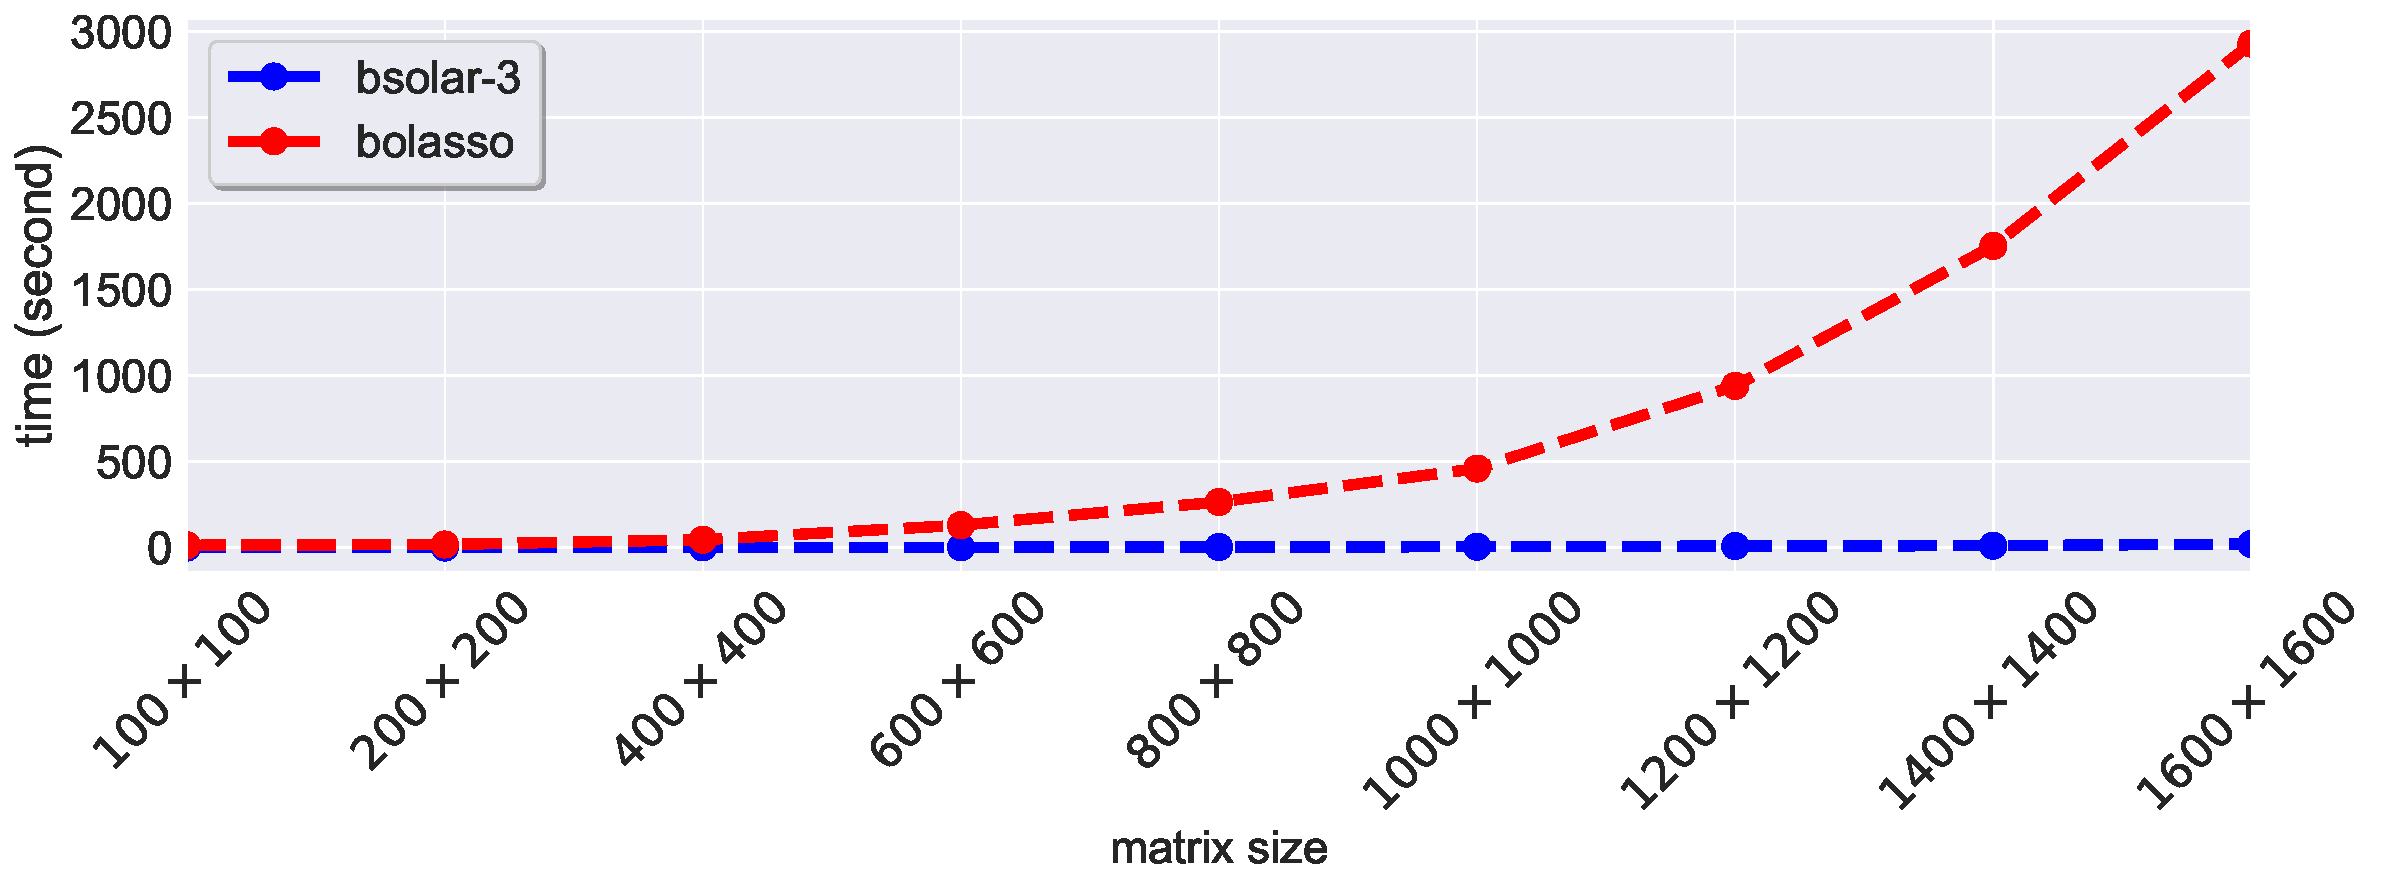
\includegraphics[width=0.8\linewidth]{runtime.pdf}
  %
  \caption{Average runtime (per pathwise coordinate descent) comparison for different $X$ matrix sizes.}
  %
  \label{fig:runtime}
  %
\end{figure}

Nonetheless, bolasso still requires a large computation time with $p/n=1200/600$ due to the $256$ CV-lasso repetitions, once again confirming the bsolar computation advantage. Figure~\ref{fig:runtime} plots average runtime against the size of the $X$ matrix. As matrix size increases, bsolar runtime increases linearly while bolasso rises exponentially, confirming the bsolar-3 advantage for high-dimensional data.

\section{Real-world data: Sydney house price prediction\label{section:application}}

To demonstrate that the improvements from solar are empirically feasible, we apply solar to real-world data. The real-world data reflect both the $p/n\rightarrow0$ scenarios as well as the challenging IRC settings, complicated dependence structures, and grouping effects typical of data in the social sciences.

The database is assembled from multiple sources. The primary source comprises real estate market transaction data for 11,974 Sydney, Australia, houses sold in 2010, including price and house attribute information (GIS coordinates, property address, bedrooms, bathrooms, car spaces, etc.). Each property is GIS-matched with: 2011 census data by Statistical Area Level 1 (the smallest census area in Australia, comprising at most 200 people or 60 households); 2010 and 2011 crime data by suburb; 2010 geo-spatial information on topology, climate, pollution, and aircraft noise; Google Maps data; 2009 primary and secondary school data; and 2010 Sydney traffic and public transport data (bus routes, train stations, and ferry wharfs). We predict house price with a linear model.

Using an ensemble of Bayes network learning algorithms for data cleaning, we reject variables with both very low conditional and unconditional correlations to house price. The remaining variables are listed in the first column of Table~\ref{table:house_variable}.\footnote{Due to the 200GB size of the database, we include only the data for these variables in the supplementary file.} The 57 variables fall into 5 broad categories: house attributes, distance to key locations (public transport, shopping, etc.), neighbourhood socioeconomic data, localized administrative and crime data, and local school quality. Pairwise correlations among all 57 covariates indicate, not surprisingly, severe multicollinearity and grouping effects, implying a harsh IRC setting.\footnote{Correlations and IRC are also reported in supplementary files.} Thus, heuristically increasing the value of the tuning parameter in lasso-type estimators (e.g., using the one-sd or the `elbow' rule) is unlikely to be useful since it may trigger further grouping effects and the random dropping of variables.

Table~\ref{table:house_variable} shows the selection comparison across the elastic net, lasso, and solar. With all variables in linear form, both lasso and elastic net lose sparsity, likely due to the complicated dependence structures and severe multicollinearity in the data, accordant with \citet{jia2010model}. By contrast, solar returns a much sparser model, with only $9$ variables selected from $57$. Very similar results are found with the variables in log form, hinting that solar possesses superior selection sparsity and robustness to a change in functional form. More importantly, solar variable selection outperforms the lasso-type estimators in terms of the balance between sparsity and prediction power. While pruning 25-48 variables from the elastic net and lasso selections, the post-selection regression $\mathrm{R}^2$ for solar falls by just 3-5\%.

%%%%%%%%%%%%%%%%%%%%%%%%%%%%%%%%%%
%%%%%%%%%%% Conclusion %%%%%%%%%%%
%%%%%%%%%%%%%%%%%%%%%%%%%%%%%%%%%%

\section{Conclusion}

\hlgreen{In this paper} we propose a new algorithm for high-dimensional data called solar (subsample-ordered least-angle regression). We show that solar yields substantial improvements over lasso in terms of the sparsity, stability, accuracy, and robustness of variable selection. We also illustrate analogous improvements from solar ensembles relative to lasso ensembles.

Detection of weak signals is a potential weakness evident in solar, although relative to the lasso competitor the difference is very slight. Nonetheless, we are working on an extension to solar, the double-bootstrap solar (DBsolar), which, if early results are any indication, promises to enable solar accurately to detect variables with weak signals.

%%%%%%%%%%%%%%%%%%%%%%%%%%%%%%%%%%
%%%%%%%%%%% References %%%%%%%%%%%
%%%%%%%%%%%%%%%%%%%%%%%%%%%%%%%%%%

\bibliographystyle{elsarticle-harv}
%\bibliographystyle{CJE}

\bibliography{ref/CVrefs}

\begin{table}[H]
  %
  \centering
  %
  \small
  %
  \caption{Variable selection results for linear and log house price models. \label{table:house_variable}}
  %
  \resizebox*{!}{0.95\textheight}{%
  \renewcommand{\arraystretch}{0.6}
  \begin{tabular}{@{}ll@{\extracolsep{6pt}}c@{\extracolsep{-2pt}}c@{\extracolsep{6pt}}c@{\extracolsep{-2pt}}c@{\extracolsep{6pt}}c@{\extracolsep{-2pt}}c@{}}
    %
    \toprule
    %
            &             & \multicolumn{2}{c}{elastic net}
                          & \multicolumn{2}{c}{lasso}
                          & \multicolumn{2}{c}{solar} \\
                          \cline{3-4} \cline{5-6} \cline{7-8} \\[-7pt]
    %
    Variable & Description& \multicolumn{1}{c}{linear}
                          & \multicolumn{1}{c}{log}
                          & \multicolumn{1}{c}{linear}
                          & \multicolumn{1}{c}{log}
                          & \multicolumn{1}{c}{linear}
                          & \multicolumn{1}{c}{log} \\
    %
    \midrule
    %
    Bedrooms           & property, number of bedrooms             & \checkmark  & \checkmark  & \checkmark  & \checkmark  & \checkmark & \checkmark  \\
    %
    Baths              & property, number of bathrooms            & \checkmark  & \checkmark  & \checkmark  & \checkmark  & \checkmark & \checkmark  \\
    %
    Parking            & property, number of parking spaces       & \checkmark  & \checkmark  & \checkmark  & \checkmark  & \checkmark & \checkmark  \\
    %
    AreaSize           & property, land size                      & \checkmark  & \checkmark  & \checkmark  & \checkmark  &   &    \\ \midrule
    %
    Airport            & distance, nearest airport                & \checkmark  & \checkmark  & \checkmark  & \checkmark  &   &    \\
    %
    Beach              & distance, nearest beach                  & \checkmark  & \checkmark  & \checkmark  & \checkmark  & \checkmark & \checkmark  \\
    %
    Boundary           & distance, nearest suburb boundary        & \checkmark  & \checkmark  & \checkmark  & \checkmark  &   &    \\
    Cemetery           & distance, nearest cemetery               & \checkmark  &             & \checkmark  &    &   &    \\
    %
    Child care         & distance, nearest child-care centre      & \checkmark  & \checkmark  & \checkmark  & \checkmark  &   & \checkmark  \\
    %
    Club               & distance, nearest club                   & \checkmark  & \checkmark  & \checkmark  & \checkmark  &   &    \\
    %
    Community facility & distance, nearest community facility     & \checkmark  & \checkmark  &    &    &   &    \\
    %
    Gaol               & distance, nearest gaol                   & \checkmark  & \checkmark  &    &    & \checkmark & \checkmark  \\
    %
    Golf course        & distance, nearest golf course            & \checkmark  & \checkmark  & \checkmark  & \checkmark  &   &    \\
    %
    High               & distance, nearest high school            & \checkmark  & \checkmark  & \checkmark  & \checkmark  &   &    \\
    %
    Hospital           & distance, nearest general hospital       & \checkmark  & \checkmark  &    & \checkmark  &   &    \\
    %
    Library            & distance, nearest library                & \checkmark  &             & \checkmark  &    &   &    \\
    %
    Medical            & distance, nearest medical centre         & \checkmark  & \checkmark  &    & \checkmark  &   &    \\
    %
    Museum             & distance, nearest museum                 & \checkmark  & \checkmark  & \checkmark  & \checkmark  &   &    \\
    %
    Park               & distance, nearest park                   & \checkmark  & \checkmark  & \checkmark  &    &   &    \\
    %
    PO                 & distance, nearest post office            & \checkmark  & \checkmark  &    & \checkmark  &   &    \\
    %
    Police             & distance, nearest police station         & \checkmark  & \checkmark  & \checkmark  & \checkmark  &   &    \\
    %
    Pre-school         & distance, nearest preschool              & \checkmark  & \checkmark  & \checkmark  & \checkmark  &   &    \\
    %
    Primary            & distance, nearest primary school         & \checkmark  & \checkmark  & \checkmark  & \checkmark  &   &    \\
    %
    Primary High       & distance, nearest primary-high school    & \checkmark  & \checkmark  & \checkmark  & \checkmark  &   &    \\
    %
    Rubbish            & distance, nearest rubbish incinerator    & \checkmark  & \checkmark  & \checkmark  &    &   &    \\
    %
    Sewage             & distance, nearest sewage treatment       & \checkmark  &    &    &    &   &    \\
    %
    SportsCenter       & distance, nearest sports centre          & \checkmark  & \checkmark  & \checkmark  & \checkmark  &   &    \\
    %
    SportsCourtField   & distance, nearest sports court/field     & \checkmark  &             & \checkmark  & \checkmark  &   &    \\
    %
    Station            & distance, nearest train station          & \checkmark  &             & \checkmark  &    &   &    \\
    %
    Swimming           & distance, nearest swimming pool          & \checkmark  & \checkmark  & \checkmark  & \checkmark  &   &    \\
    %
    Tertiary           & distance, nearest tertiary school        & \checkmark  & \checkmark  & \checkmark  & \checkmark  &   &    \\
    %
    \midrule
    %
    Mortgage           & SA1, mean mortgage repayment (log)       & \checkmark  & \checkmark  & \checkmark  & \checkmark  & \checkmark & \checkmark  \\
    %
    Rent               & SA1, mean rent (log)                     & \checkmark  & \checkmark  & \checkmark  & \checkmark  & \checkmark & \checkmark  \\
    %
    Income             & SA1, mean family income (log)            & \checkmark  & \checkmark  & \checkmark  & \checkmark  & \checkmark & \checkmark  \\
    %
    Income (personal)  & SA1, mean personal income (log)          & \checkmark  &    &    &    &   &    \\
    %
    Household size     & SA1, mean household size                 & \checkmark  & \checkmark  & \checkmark  & \checkmark  &   &    \\
    %
    Household density  & SA1, mean persons to bedroom ratio       & \checkmark  & \checkmark  & \checkmark  & \checkmark  &   &    \\
    %
    Age                & SA1, mean age                            & \checkmark  & \checkmark  & \checkmark  & \checkmark  &   & \checkmark  \\
    %
    English spoken     & SA1, percent English at home             & \checkmark  &             & \checkmark  &    &   &    \\
    %
    Australian born    & SA1, percent Australian-born             & \checkmark  &             & \checkmark  &    &   &    \\
    %
    \midrule
    %
    Suburb area        & suburb area                             & \checkmark  &    & \checkmark  & \checkmark  &   &    \\
    %
    Population         & suburb population                       & \checkmark  & \checkmark  &    & \checkmark  &   &    \\
    %
    TVO2010            & suburb total violent offences, 2010     & \checkmark  &             &    &    &   &    \\
    %
    TPO2010            & suburb total property offences, 2010    & \checkmark  & \checkmark  &    & \checkmark  &   &    \\
    %
    TVO2009            & suburb total violent offences, 2009     & \checkmark  & \checkmark  & \checkmark  &    &   &    \\
    %
    TPO2009            & suburb total property offences, 2009    & \checkmark  & \checkmark  &    &    &   &    \\
    %
    \midrule
    %
    ICSEA              & local school, socio-educational advantage & \checkmark  & \checkmark  & \checkmark  & \checkmark  & \checkmark & \checkmark  \\
    %
    ReadingY3          & local school, year 3 mean reading score  & \checkmark  & \checkmark  & \checkmark  & \checkmark  &   &    \\
    %
    WritingY3          & local school, year 3 mean writing score  & \checkmark  & \checkmark  & \checkmark  & \checkmark  &   &    \\
    %
    SpellingY3         & local school, year 3 mean spelling score & \checkmark  & \checkmark  & \checkmark  &    &   &    \\
    %
    GrammarY3          & local school, year 3 mean grammar score  & \checkmark  &             & \checkmark  &    &   &    \\
    %
    NumeracyY3         & local school, year 3 mean numeracy score & \checkmark  & \checkmark  & \checkmark  & \checkmark  &   &    \\
    %
    ReadingY5          & local school, year 5 mean reading score  & \checkmark  &    &    &    &   &    \\
    %
    WritingY5          & local school, year 5 mean writing score  & \checkmark  & \checkmark  & \checkmark  &    &   &    \\
    %
    SpellingY5         & local school, year 5 mean spelling score & \checkmark  & \checkmark  & \checkmark  &    &   &    \\
    %
    GrammarY5          & local school, year 5 mean grammar score  & \checkmark  & \checkmark  & \checkmark  &    &   &    \\
    %
    NumeracyY5         & local school, year 5 mean numeracy score & \checkmark  &             &    &    &   &    \\
    %
    \midrule
    %
                      & Number of variables selected  & 57 & 45 & 44 & 36 & 9 & 11 \\
                      & post-selection OLS $R^2$      & 0.55 & 0.76 & 0.55 & 0.76 & 0.50 & 0.73\\
                      & Sample size & \multicolumn{6}{c}{11,974} \\

    \bottomrule

  \end{tabular}}

\end{table}

\clearpage
\begin{appendices}
\section{$L_0$ path ranking accuracy and variable selection consistency}

For generality, we derive the theoretical properties of solar under the general forward selection framework of \citet[Figure~1]{zhang09}. Our proof method is summarized as follows. Under various settings and assumptions, \citet{tropp2004greed}, \citet{yuan2007non}, \citet{wainwright2009sharp}, \citet{zhang09}, and \citet{ing2011stepwise} have shown: (i) forward selection is consistent in different modes, and (ii) informative variables are ranked higher at earlier stages of the solution path than redundant variables. Since the $L_0$ path on each solar subsample is essentially the re-parameterized forward selection path, (i) and (ii) can be applied directly to the $L_0$ path on each solar subsample. As a result, we can build a probabilistic lower bound to show that, on average, (i) and (ii) also hold for the average $L_0$ path and for the variable selection result on the average $L_0$ path (including solar variable selection). \hl{We follow the methods of} \citet{tropp2004greed}, \citet{wainwright2009sharp}, and \citet{zhang09}, \hl{since their assumptions and analysis methods are similar to the theoretical analysis of lasso-type estimators.} We follow the \citet{zhang09} notation.

\begin{definition}
  Consider the regression model $Y = X\beta + \mathbf{e}$, \label{def:notation}
\end{definition}
%
\begin{enumerate}
  %
  \item     $Y = \left[ y_1, \ldots, y_n \right]^T \in \mathbb{R}^{n \times 1}$ is the response variable.

  \item     The data matrix is $X = \left[ \mathbf{x}_1, \ldots,\mathbf{x}_p \right] \in \mathbb{R}^{n \times p}$ with columns $\mathbf{x}_j \in \mathbb{R}^{n \times 1}$, $\forall j=1,\ldots,p$, and rows $ X_{i,\bigcdot} \in \mathbb{R}^{1 \times p}$, $\forall i = 1,\ldots,n$. $\mathbf{e}\in \mathbb{R}^{n\times 1}$ is a stochastic noise term.
  %
  \item     The regression coefficients of the data generating process (DGP) are $\overline{\beta} = \left[\,\overline{\beta}_1, \ldots, \overline{\beta}_{p_1}, \mathbf{0} \right]^T \in \mathbb{R}^{p\times 1}$, where the first $p_1$ entries are not $0$.
  %
  \item     The support, $\forall \beta \in \mathbb{R}^{p \times 1}$, is $\mathrm{supp}(\beta) = \{ j : \beta_j \neq 0 \} $.
  %
  \item     Given $X \in \mathbb{R}^{n \times p}$ and $F \subset \left\{1, \ldots, p \right\}$,
  %
  \begin{displaymath}
    %
    \widehat{\beta}_{X} \left( F,Y \right) =
    \mathrm{argmin}_{ \beta \in \mathbb{R}^{p \times 1}} \;\;
    \frac{1}{n}\left\Vert X\beta - Y\right\Vert_{2}^{2}
    \quad\mbox{subject to}\quad \mathrm{supp}(\beta)\subset F.
    %
  \end{displaymath}
  %
  That is, $\widehat{\beta}_{X}\left(F,Y\right)$ is the least squares solution with coefficients restricted to $F$.
  %
  \item $\left\vert F \right\vert$ is the cardinality of $F$ while $\overline{F}-F$ is the difference of sets $\overline{F}$ and $F$.
  %
  \item $X_F$ is an $n \times \left\vert F \right\vert$ matrix with columns $\mathbf{x}_j \in \left[ \mathbf{x}_0, \ldots \mathbf{x}_p \right]$ with $j\in F$ arranged in ascending order.
  %
  \item To introduce the irrepresentable condition and sparse eigenvalue condition, define
  %
  \begin{displaymath}
    %
    \mu_{X}\left(F\right)=\max_{j\in F}\left\Vert \left(X_{F}^{T}X_{F}\right)^{-1}X_{F}^{T}\mathbf{x}_{j}\right\Vert _{1}
    %
  \end{displaymath}
  %
  and
  %
  \begin{displaymath}
    %
    \rho_{X}\left(F\right)=\inf\left\{ \frac{1}{n}\left\Vert X\beta\right\Vert _{2}^{2}/\left\Vert \beta\right\Vert _{2}^{2}:\mathrm{supp}\left(\beta\right)\subset F\right\}
    %
  \end{displaymath}
  %
  \item (The $\epsilon$ stopping rule.) The \citet[Figure~1]{zhang09} framework is also known as orthogonal matching pursuit (OMP). Prior to stage $l$, forward selection finds the unselected variable
  %
  \begin{displaymath}
    %
    \mathbf{x}^{(l)} = \mathrm{argmax}_{\mathbf{x}_j} \;\; \left\vert \mathbf{x}_j^T u^{(l-1)} \right\vert, \\
    \quad\mbox{for all unselected }\mathbf{x}_{j},
    %
  \end{displaymath}
  %
  where $u^{\left(l-1\right)}$ is the forward regression residual of stage $l-1$. If $\left\vert (\mathbf{x}^{(l)})^T u^{(l-1)} \right\vert > \epsilon$, the forward selection loop will select $\mathbf{x}^{(l)}$, compute $u^{(l)}$ and move to stage $l+1$; otherwise, the forward selection loop will stop and report the regression coefficients and selected variables on and before stage $l-1$.
\end{enumerate}

We also adopt the \citet{zhang09} assumptions:
%
\begin{description}
  %
  \item [{[}A1{]}] each $\mathbf{x}_i$ is normalized such that $\left\Vert \mathbf{x}_{j}\right\Vert _{2}^{2}/n=1,\;\forall j=1,\ldots,p$;
  %
  \item [{[}A2{]}] the $\overline{\beta}$ is sparse: $\exists \overline{\beta} \in \mathbb{R}^{p\times 1}$ with $\overline{F} = \mathrm{supp} \left( \overline{\beta} \right)$ such that $ \mathbf{E} \left( Y \right) = X\overline{\beta} = \left[ X_{1,\bigcdot} \; \overline{\beta}, \;  \ldots, \; X_{n,\bigcdot} \; \overline{\beta} \right]^T$;
  %
  \item [{[}A3{]}] the irrepresentable condition \citep{tropp2004greed}: $\mu_{X}\left(\overline{F}\right)<1$; the sparse eigenvalue condition \citep{wainwright2009sharp}: $\rho_{X}\left(\overline{F}\right)>0$.
  %
  \item [{[}A4{]}] there exists a $ \sigma > 0$ such that $Y = \left[ Y_1, \ldots, Y_n \right]$ are independent (but not necessarily identically distributed) sub-Gaussians with $\mathbb{E} \left(Y_i\right)=  X_{i,\bigcdot} \; \overline{\beta}$ and $\mathbb{E}_{Y_i} \left( e^{t\left(Y_i - \mathbb{E} \left( Y_i \right) \right)}\right) \leqslant e^{\sigma^2t^2/2}$, $\forall t\in \mathbb{R}$ and $\forall i\in \left\{1,\ldots,n\right\}$.
\end{description}

\textbf{A4} implies that $Y$ can be either bounded or unbounded. \textbf{A2} and \textbf{A4} imply that the regression noise in the DGP, $\left[e_1, \ldots, e_n\right]^T$, are independent sub-Gaussians.

The proof of variable selection accuracy and variable ranking accuracy is specified in the following steps.

%%%%%%%%% step 1 %%%%%%%%%

\subsection*{Step 1 : re-parameterize the $\epsilon$ stopping rule via $\widehat{q}^k$ }

\citet[Theorem 1]{zhang09} shows that the probability of omitting informative variables is bounded on a finite sample.
%
\begin{theorem}
  %
  \label{theoremA1}
  \citep{zhang09} Consider the forward selection algorithm with Assumption 1 satisfied. Given any $\eta \in \left( 0, 1 \right)$, with probability larger than $1 - \eta$, if the $\epsilon$  stopping criterion stops forward selection at stage $l$, satisfying
  %
  \begin{equation}
    %
    \epsilon>\frac{1}{1-\mu_X \left( \overline{F} \right)} \sigma\sqrt{ 2 \ln \left( 4p / \eta \right)}
    %
  \end{equation}
  %
  and
  %
  \begin{equation}
    %
    \min_{j\in\overline{F}}\left|\overline{\beta}_{j}\right|\geqslant\frac{3\epsilon}{\rho_{X}\left(\overline{F}\right)\cdot\sqrt{n}}, \label{thm0}
    %
  \end{equation}
  %
  then when the procedure stops at stage $l$,
  %
  \begin{equation}
    %
    \overline{F}=F^{\left(l-1\right)}, \nonumber
    %
  \end{equation}
  %
  where $F^{\left(l-1\right)}$ is the set of variable selected at stage $l-1$. $\blacksquare$
  %
\end{theorem}

As shown in Definition~\ref{def:notation}, \citet{zhang09} executes each forward selection stage using $\epsilon$. By contrast, we re-parameterize forward selection stages (in Algorithm 1) and the stopping rule (in Algorithm 2) using $\widehat{q}$. Given the assumption $\epsilon > \frac{1}{1-\mu_X \left( \overline{F} \right)} \sigma\sqrt{ 2 \ln \left( 4p / \eta \right)}$, we can find an equivalent stopping criterion based on $\widehat{q}$ as follows,

\begin{itemize}
  %
  \item Assume that, on subsample $\left(Y^{k},X^{k}\right)$, $\epsilon>\frac{1}{1-\mu_{X}\left(F\right)}\sigma\sqrt{2\ln\left(4p/\eta\right)}$ stops the forward selection at stage $l^{k}$;
  %
  \item from line 6 of Algorithm 1, variables selected before stage $l^{k}$ must have $\widehat{q}_i^k$ values $> \left(\widetilde{p} + 1 - l^k \right) / \widetilde{p}$, where $\widetilde{p} = \min\left\{ n(K-1)/K, p\right\}$
  %
  \item hence, on the $k$\textsuperscript{th} subsample, the stopping rule
  %
  \begin{displaymath}
    %
    \mbox{forward selection stops at stage } l^k
    %
  \end{displaymath}
  %
  is equivalent to the stopping rule
  %
  \begin{displaymath}
    %
    \mbox{forward selection only selects the variables } \left\{ \mathbf{x}_j:\widehat{q}_j^k>\left(\widetilde{p}+1-l^k\right)/\widetilde{p}\right\}.
    %
  \end{displaymath}
  %
\end{itemize}
\medskip

\citet{zhang09} also assumes that, when forward selection stops at stage $l^k$ on subsample $\left(Y^{k},X^{k}\right)$,
%
\begin{displaymath}
  %
  \epsilon>\frac{1}{1-\mu_{X}\left(F\right)}\sigma\sqrt{2\ln\left(4p/\eta\right)},
  \;\exists\; \eta \in \left(0, 1\right).
  %
\end{displaymath}
%
The assumption plays a key role for true signal recovery. Since solar does not explicitly use $\epsilon$, we need to re-parameterize the assumption before applying the \citet{zhang09} result. Specifically, denote
%
\begin{equation}
  %
  \omega^{\left(l^k\right)} = \left\vert \left( \mathbf{x}^{\left( l^k \right)}\right) ^T u^{\left(l^k \right)} \right\vert,
  %
\end{equation}
%
where $u^{\left( l^k \right)}$ is the regression residual and $\mathbf{x}^{ \left( l^k \right)}$ the variable selected at stage $l^k$. Solar selects variables on the $L_0$ and average $L_0$ paths based on $\widehat{q}^k$ and $\widehat{q}$. Hence, we can analyze the selection decisions of solar by examining the absolute co-movement between $u^{\left( l^k \right)}$ and $\mathbf{x}^{ \left( l^k \right)}$ on the $L_0$ path, which is identical to the $\epsilon$ assumption. This can be shown as follows.
%
\begin{itemize}
  %
  \item Assume the $\epsilon$ stopping rule stops forward selection at stage $l^k$ and $\epsilon > \frac{1}{1-\mu_{X}\left(F\right)}\sigma\sqrt{2\ln\left(4p/\eta\right)}$. We must have
  %
  \begin{equation}
    %
    \omega^{\left(l^k - 1\right)} > \epsilon > \frac{1}{1 - \mu_X \left( F \right)} \sigma \sqrt{ 2 \ln \left(4p / \eta \right)}
    %
  \end{equation}
  Hence, stopping forward selection based on $\epsilon > \frac{1}{1 - \mu_X \left( F \right)} \sigma \sqrt{ 2 \ln \left(4p / \eta \right)}$ implies
  \begin{displaymath}
    \omega^{\left(l^k - 1\right)} > \frac{1}{1 - \mu_X \left( F \right)} \sigma \sqrt{ 2 \ln \left(4p / \eta \right)}.
  \end{displaymath}
  %
  \item Assume $\omega^{\left(\bigcdot\right)} > \frac{1}{1 - \mu_X \left( F \right)} \sigma \sqrt{ 2 \ln \left(4p / \eta \right)}$ is not violated until stage $l^k$. This implies that we have $\omega^{\left(l^k - 1 \right)} > \frac{1}{1 - \mu_X \left( F \right)} \sigma \sqrt{ 2 \ln \left(4p / \eta \right)}$. Besides, since $\omega^{\left(\bigcdot\right)} > \frac{1}{1 - \mu_X \left( F \right)} \sigma \sqrt{ 2 \ln \left(4p / \eta \right)}$ for the first $l^k-1$ stages, there exists some $\epsilon^*$ such that 
  %
  \begin{equation}
    %
    \epsilon^* \in \left( \frac{1}{1 - \mu_X \left( F \right)} \sigma \sqrt{ 2 \ln \left(4p / \eta \right)} \; , \; \min_{i < l^k} \; \omega^{\left( i \right)} \right) \label{eqn:omega_epsilon}
    %
  \end{equation}
  %
  If we equip the $\epsilon$ stopping rule with the $\epsilon^*$, the $\epsilon$ stopping rule will also stop forward selection at stage $l^k$.
  %
\end{itemize}
\medskip

\noindent
Hence, `the $\epsilon > \frac{1}{1 - \mu_X \left( F \right)} \sigma \sqrt{ 2 \ln \left(4p / \eta \right)}$ stopping rule stops forward selection at stage $l^k$' is equivalent to `the last variable that forward selection selects before stop has its $\omega$ larger than $\frac{1}{1-\mu_{X}\left(F\right)}\sigma\sqrt{2\ln\left(4p/\eta\right)}$'. As such, we can re-parameterize the stopping rule on $\left(Y^{k},X^{k}\right)$ based on $\widehat{q}_{i}^{k}$ as follows
%
\begin{definition}
  (The $\epsilon$ and $\widetilde{q}^k$ stopping assumptions) \label{def:stopping assumption}
\end{definition}

\begin{itemize}
  %
  \item We refer to the \citet{zhang09} assumption on $\epsilon$ stopping rule as \emph{the $\epsilon$ stopping assumption}:
  %
  \begin{eqnarray}
    %
    \mbox{when forward selection stops at stage } l^k \mbox{ on subsample } \left(Y^k, X^k\right), \\ \notag
    \exists \eta \in \left( 0, 1\right) \mbox{ such that }\epsilon>\frac{1}{1-\mu_{X}\left(F\right)}\sigma\sqrt{2\ln\left(4p/\eta\right)}.
    %
  \end{eqnarray}
  %
  \item Assume forward selection only selects $\left\{ \mathbf{x}_j:\widehat{q}_j^k > \frac{\widetilde{p} + 1 - l^k} {\widetilde{p}} \right\}$ on subsample $\left(Y^k, X^k \right)$. We define 
  %
  \begin{displaymath}
    %
    \omega^{\left(l^k\right)} = \left\vert \left( \mathbf{x}^{\left( l^k \right)}\right) ^T u^{\left(l^k \right)} \right\vert.
    %
  \end{displaymath}
  %
  For simplicity, we denote $\omega$ as $\omega^{\left( \bigcdot \right)}$ of the last variable that forward selection selects.
  %
  \item we refer to the following equivalent assumption for solar as \emph{the $\widetilde{q}^k$ stopping assumption}:
  %
  \begin{align}
    %
    \mbox{when forward selection only selects } \left\{ \mathbf{x}_j:\widehat{q}_j^k > \frac{\widetilde{p} + 1 - l^k} {\widetilde{p}} \right\} \mbox{ on } \left(Y^k, X^k \right), \notag \\
    %
    \exists\, \eta \in \left( 0, 1\right) \mbox{ such that } \omega >\frac{1}{1-\mu_{X}\left(F\right)}\sigma\sqrt{2\ln\left(4p/\eta\right)}. \label{eqn:qk_stopping}
    %
  \end{align}
  %
\end{itemize}
\medskip

Based on Definition~\ref{def:stopping assumption}, we can re-parameterize Theorem~\ref{theoremA1} into Lemma~\ref{lemma:1}.

\begin{lemma}
  %
  Consider the forward selection algorithm on the $k$th subsample $\left(Y^{k},X^{k}\right)$ with Assumption 1 satisfied. With probability larger than $1-\eta$, if (\ref{eqn:qk_stopping}) is satisfied and
  \begin{displaymath}
      \min_{j\in\overline{F}}\left|\overline{\beta}_{j}\right|\geqslant\frac{3\omega}{\rho_{X}\left(\overline{F}\right)\cdot\sqrt{n\left(K-1\right)/K}},
  \end{displaymath}
  then
  \begin{displaymath}
      \overline{F}=\left\{ \mathbf{x}_{j}:\widehat{q}_{i}^{k}>\widetilde{q}^{k}\right\}.
  \end{displaymath}
  %
  where $\widetilde{q}^k = \left(\widetilde{p} + 1 - l^k\right) / \widetilde{p}$.
  %
  \label{lemma:1}
  %
\end{lemma}

\begin{proof}
    %
  Lemma~\ref{lemma:1} is derived by replacing the $\epsilon$ stopping assumption with the $\widehat{q}^k$ stopping assumption. Note that
  \begin{displaymath}
    \min_{j\in\overline{F}}\left|\overline{\beta}_{j}\right|\geqslant\frac{3\omega}{\rho_{X}\left(\overline{F}\right)\cdot\sqrt{n\left(K-1\right)/K}} \implies \min_{j\in\overline{F}}\left|\overline{\beta}_{j}\right| \geqslant \frac{3\epsilon}{\rho_{X}\left(\overline{F}\right)\cdot\sqrt{n\left(K-1\right)/K}},
\end{displaymath}
since (\ref{eqn:omega_epsilon}) implies that $\exists \epsilon > \frac{1}{1-\mu_{X}\left(F\right)}\sigma\sqrt{2\ln\left(4p/\eta\right)}$ such that $\omega > \epsilon$.  We also replace $n$ in (\ref{thm0}) with $n\left(K-1\right)/K$ since each subsample randomly drops $1/K$ of the original sample points in Algorithm 1.
    %
\end{proof}
\medskip

%%%%%%%%%%%% step 2 %%%%%%%%%%%%

\subsection*{Step 2 : averaging performance}

Since we assume the nonzero $\overline{\beta}_i$ are the first $p_1$ components of $\overline{\beta}$, x can be rewritten as
%
\begin{lemma}
  Consider the forward selection algorithm on the $k$th subsample $\left(Y^{k},X^{k}\right)$ with Assumption 1 satisfied. With probability less than $\eta$, if (\ref{eqn:qk_stopping}) is satisfied and
  \[
      \min_{j\in\overline{F}}\left|\overline{\beta}_{j}\right|\geqslant\frac{3\omega}{\rho_{X}\left(\overline{F}\right)\cdot\sqrt{n\left(K-1\right)/K}},
  \]
  then
  \[
  \begin{cases}
      \widehat{q}_j^k \leqslant \widetilde{q}^k, \; \forall j\leqslant p_1\\
      \widehat{q}_j^k > \widetilde{q}^k, \; \forall j>p_1.
  \end{cases}
  \]
  where $\widetilde{q}^k = \left(\widetilde{p} + 1 - l^k\right) / \widetilde{p}$.
  %
  \label{lemma:2}
  %
\end{lemma}
%
\noindent
Lemma~\ref{lemma:2} \hl{direcly implies that, with large probability, you can find a theshold value $\widetilde{q}^k$ on the $L_0$ path that perfectly seperates the informative from the redundant.}

To accommodate multiple subsamples in the average $L_0$ path, we define the $\widehat{q}$ stopping rule by slightly modifying (\ref{eqn:qk_stopping}).
%
\begin{definition}
  (The assumption for the $\widetilde{q}$ stopping rule). We refer to the following rule as \emph{the $\widetilde{q}$ stopping assumption} for the average $L_0$ path:
  %
  \begin{eqnarray}
    %
    \mbox{when forward selection only selects } \left\{ \mathbf{x}_j:\widehat{q}_j^k > \left( \widetilde{p} + 1 - l^k \right) / \widetilde{p} \right\} \mbox{ on } \left(Y^k, X^k \right), \notag \\
    %
    \exists\, \eta \in \left( 0, 1/K\right) \mbox{ such that } \omega >\frac{1}{1-\mu_{X}\left(F\right)}\sigma\sqrt{2\ln\left( \frac{4p}{K\eta}\right)}.
    %
    \label{eqn:q_hat_stopping}
    %
  \end{eqnarray}
  %
\end{definition}
\medskip

Lemma~\ref{lemma:3} follows from the $\widetilde{q}$ stopping assumption.

\begin{lemma}
  Consider the forward selection algorithm on the average $L_{0}$ path with Assumption 1 satisfied. With probability less than $\eta$, if (\ref{eqn:q_hat_stopping}) is satisfied and
  \[
      \min_{j\in\overline{F}}\left|\overline{\beta}_{j}\right|\geqslant\frac{3\omega}{\rho_{X}\left(\overline{F}\right)\cdot\sqrt{n\left(K-1\right)/K}},
  \]
  then
  \[
  \begin{cases}
      \frac{1}{K}\sum\widehat{q}_{i}^{k}=\widehat{q}_{i}>\widetilde{q}^{*},\forall i\leqslant p_{1}\\
      \frac{1}{K}\sum\widehat{q}_{i}^{k}=\widehat{q}_{i}\leqslant\widetilde{q}^{*},\forall i>p_{1}
  \end{cases}
  \]
  where $\widetilde{q}^* = \frac{1}{n} \sum_k^K \widetilde{q}^k / K$ and $\widetilde{q}^k = \left(\widetilde{p} + 1 - l^k\right) / \widetilde{p}$.
  %
  \label{lemma:3}
  %
\end{lemma}

\begin{proof}
    The proof is a direct result from Lemma~2. If we apply the $\widetilde{q}$ stopping rule, Lemma~2 implies that
    \begin{eqnarray}
        Pr\left\{ \widehat{q}_i^k \leqslant \widetilde{q}^k,\forall i\leqslant p_1 \mbox{ and } \widehat{q}_j^k > \widetilde{q}^k,\forall j>p_1 \right\} \leqslant \eta/K.
    \end{eqnarray}
    Since, for multiple events $A_i$, $Pr\left\{ \cap_i A_i\right\} \leqslant \sum_i Pr\left\{ A_i\right\}$, we have
    \begin{eqnarray}
        Pr\left\{ \sum_{k=1}^K \widehat{q}_i^k \leqslant \sum_{k=1}^K \widetilde{q}^k,\forall i\leqslant p_1 \mbox{ and } \sum_{k=1}^K  \widehat{q}_j^k > \sum_{k=1}^K \widetilde{q}^k,\forall j>p_1 \right\} \leqslant \eta.
    \end{eqnarray}
    Since, $\widehat{q}_i = \frac{1}{K}\sum\widehat{q}_{i}^{k}$ and $\widetilde{q}^{\,*} = \frac{1}{K}\sum\widetilde{q}^k$, we have
    \begin{eqnarray}
        Pr\left\{ \widehat{q}_i \leqslant \widetilde{q}^{\,*},\forall i \leqslant p_1 \mbox{ and } \widehat{q}_j > \widetilde{q}^{\,*},\forall j>p_1 \right\} \leqslant \eta.
    \end{eqnarray}
\end{proof}
\noindent
Lemma~\ref{lemma:3} \hl{direcly implies that, with large probability, you can find a theshold value $\widetilde{q}^*$ on the average $L_0$ path that perfectly seperates the informative from the redundant.}

%%%%%%%%%%%% step 3 %%%%%%%%%%%%

\subsection*{Step 3 : variable selection consistency}

Based on Lemma~\ref{lemma:3}, Theorem~\ref{thm:1} on variable selection consistency is straightforward.

\begin{theorem}
  Consider the forward selection algorithm on the average $L_0$ path with Assumption 1 satisfied, noise $\sigma$ independent of $n$. Assume that the strong irrepresentable condition holds. For each sample size $n$, denote $F\left( n \right)$ as the index set of selected variables when forward selection stops with $\omega\geqslant n^{s/2}$, $\forall s\in(0,1]$ , and $\overline{F}\left(n\right)$ as the corresponding index set of informative variables. We have
  \[
      Pr\left(\;F\left(n\right)\neq\overline{F}\left(n\right)\;\right)\leqslant \exp\left(-\frac{n^{s}}{\log\left(n\right)}\right)
  \]
  if
  \[
      p\left(n\right)\leqslant\exp\left(\frac{n^{s}}{\log\left(n\right)}\right),
  \]
  and
  \[
      \min_{j\in\overline{F}}\left|\overline{\beta}_{j}\right|\geqslant\frac{3n^{(s-1)/2}}{\rho_{X}\left(\overline{F}\left(n\right)\right)}
  \]
  where $p\left(n\right)$ is the total dimension of variable as $n$ increases.
  %
  \label{thm:1}
  %
\end{theorem}

\begin{proof}
  When $n$ is sufficiently large, the assumptions
  \[
      \omega^{\left(l^k \right)} = \left\vert \left( \mathbf{x}^{\left( l^k \right)}\right) ^T u^{\left(l^{k}\right)} \right\vert >\frac{1}{1-\mu_{X}\left(F\right)}\sigma\sqrt{2\ln\left(4p/\eta\right)}
  \]
  and
  \[
      \min_{j\in\overline{F}}\left|\overline{\beta}_{j}\right|\geqslant\frac{3\omega}{\rho_{X}\left(\overline{F}\right)\cdot\sqrt{n\left(K-1\right)/K}}
  \]
  hold with $\eta = \exp\left(-n^s/\log(n)\right)$. Thus, Theorem~\ref{thm:1} follows from Lemma~\ref{lemma:2} and \ref{lemma:3}.
\end{proof}


\end{appendices}

\end{document}

%%%%%%%%%%%%%%%%%%%%%%%%%%%%%%%%%%%%%%%%%%%%%%%%%%%%%%%%%%%%%%%%%%%%%%%%%%%
%%%%%%%%%%%%%%%%%%%%%%%%%%%%%%%%%%%%%%%%%%%%%%%%%%%%%%%%%%%%%%%%%%%%%%%%%%%
%%%%%%%%%%%%%%%%%%%%%%%%%%%%%%%%%%%%%%%%%%%%%%%%%%%%%%%%%%%%%%%%%%%%%%%%%%%

\citet{tibshirani2015general} \hl{illustrates his point in a number of large-scale applications. We summarize two of them in Figure}~\ref{fig:intro1} and \ref{fig:intro2}.
%
\begin{itemize}
  %
  \item With $n = 200, p = 4000$, the top row of Figure~\ref{fig:intro1} \hl{shows that forward selection can achieve competitive mean squared errors to that of group lasso under two different setups for the predictors in group lasso regression: uncorrelated and block correlated. (The curves were averaged over 10 simulations, with standard deviations denoted by dotted lines.) The lower table reports runtimes in seconds (averaged over 10 simulations, with standard deviations in parentheses) for the various algorithms considered, and shows that the stagewise algorithm represents a computationally attractive alternative to the coordinate descent approach and the Frank-Wolfe algorithm.}
  %
  \item Figure~\ref{fig:intro2} \hl{compares between fused lasso and forward selection on image denoising. The true underlying $300 \times 200$ image is displayed in the middle of the top row. Over 10 noisy pertubations of this underlying image, with one such example shown in the right plot of the top row, we compare averaged mean squared errors of the exact solutions and stagewise estimates, in the left plot of the top row. Average timings for these methods are given in the bottom table. (Standard deviations are denoted by dotted lines in the error plots, and are in parentheses in the table.) The stagewise estimates have competitive mean squared errors and are fast to compute.}
  %
\end{itemize}

\begin{figure}[ht]
  %
    \centering
  %
    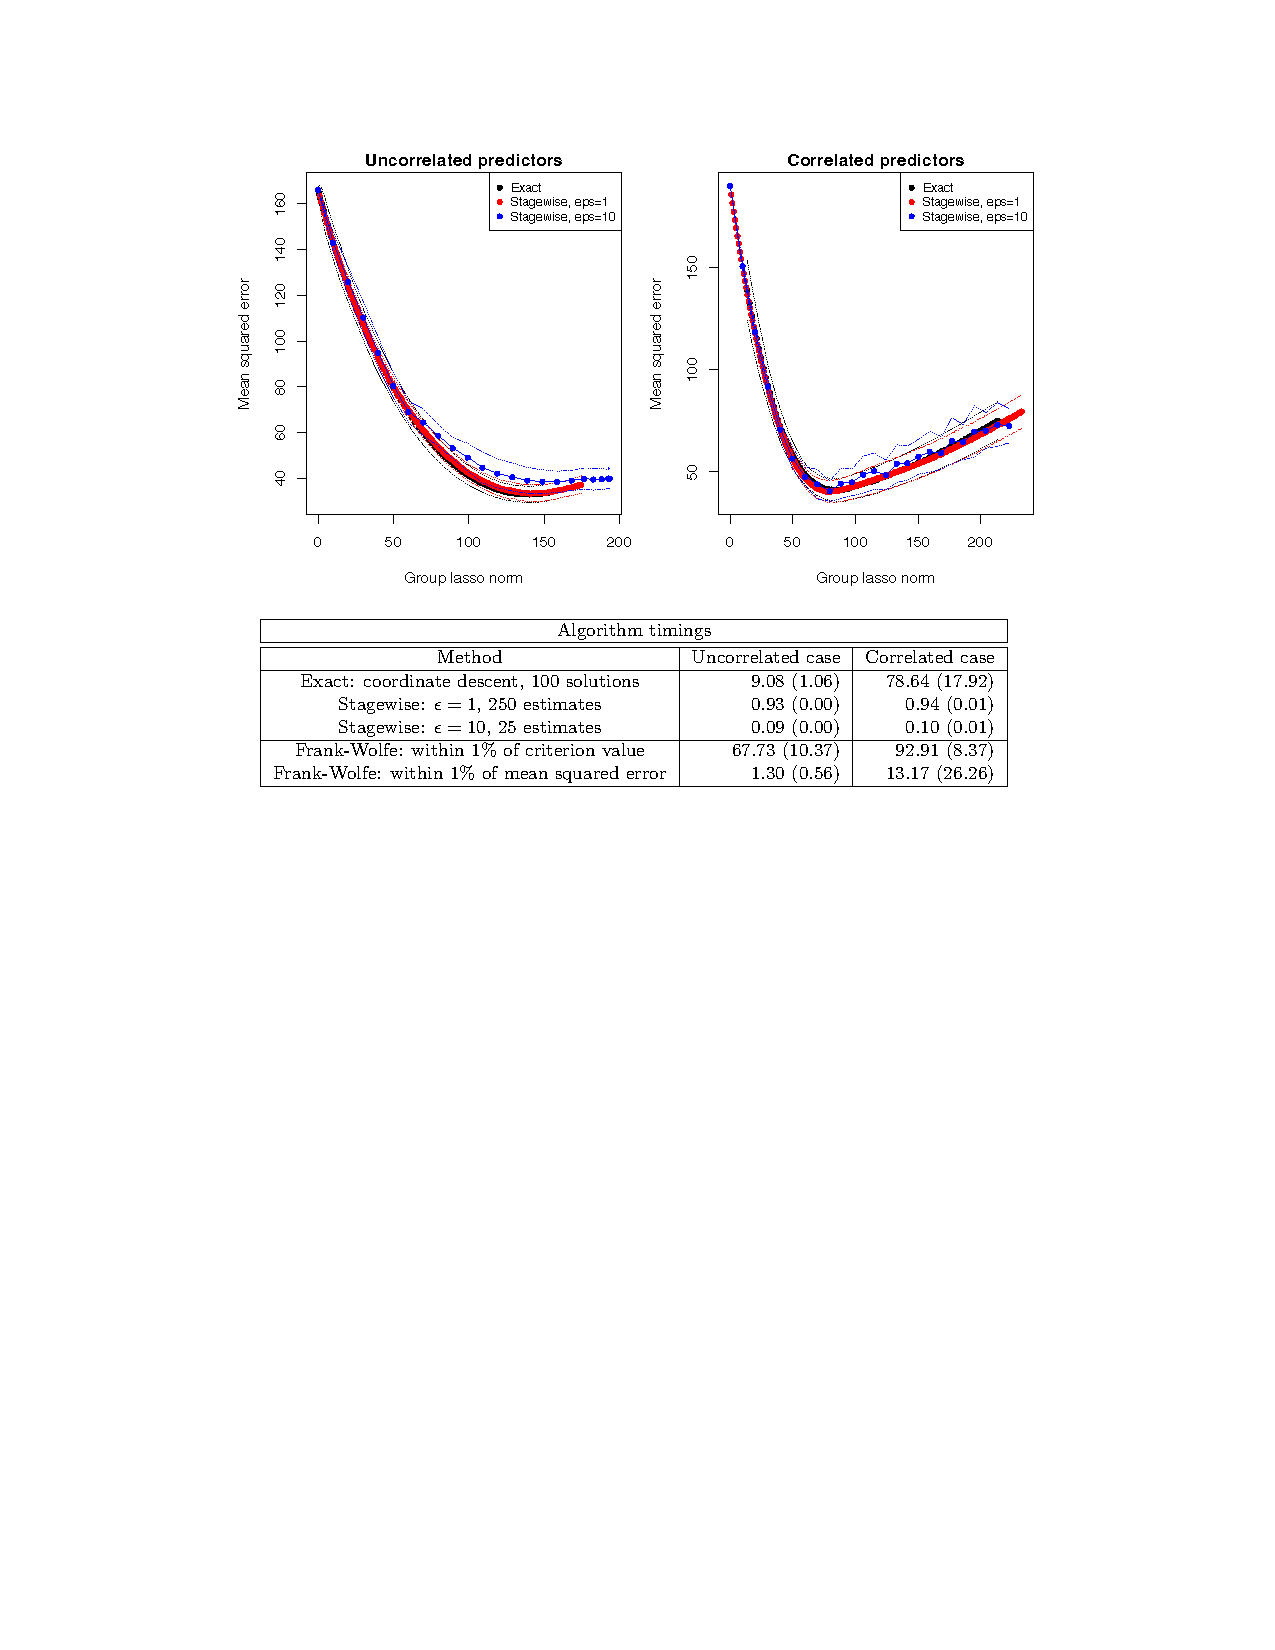
\includegraphics[width=0.66\paperwidth]{intro1.pdf}
  %
    \caption{Statistical and computational comparisons between group lasso (coordinate descent) and the forward selection with $n = 200, p = 4000$.}
  %
    \label{fig:intro1}
  %
\end{figure}

\begin{figure}[ht]
  %
    \centering
  %
    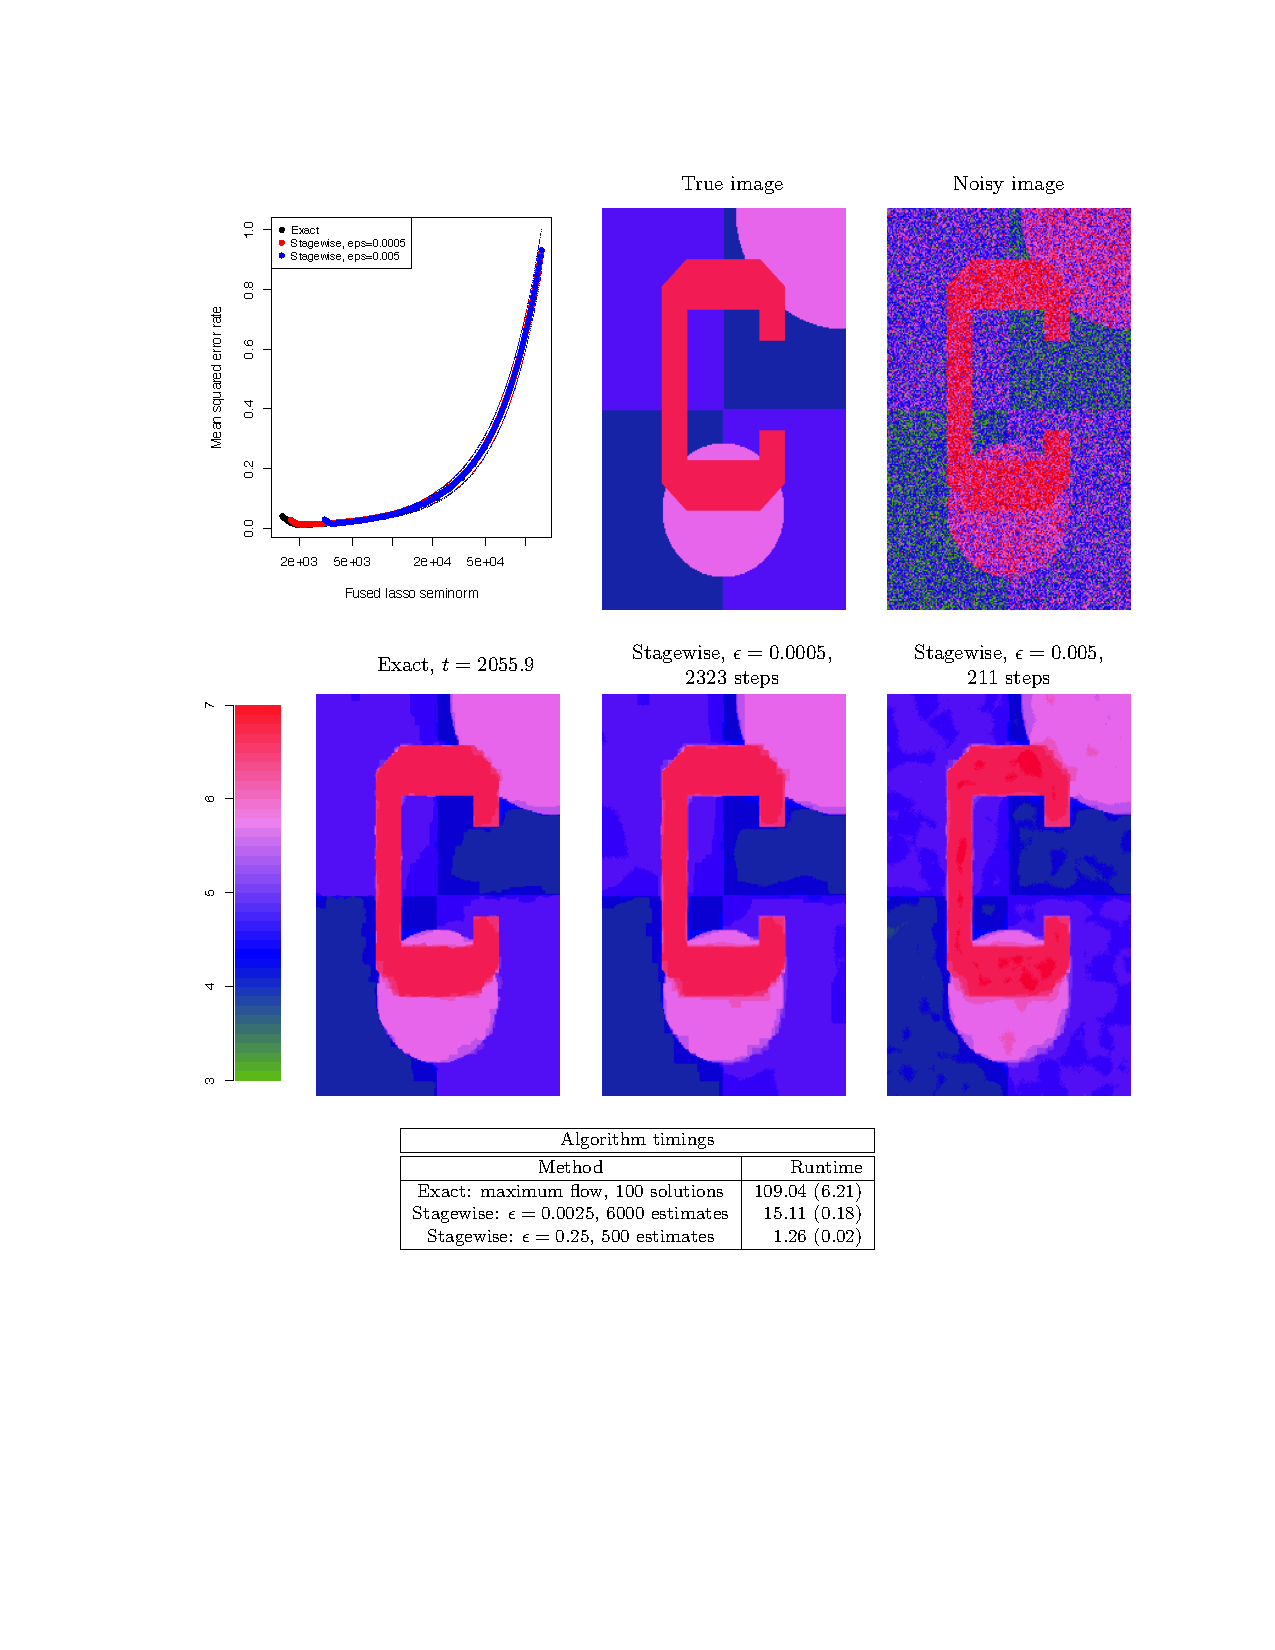
\includegraphics[width=0.55\paperwidth]{intro2.pdf}
  %
    \caption{Statistical and computational comparisons between fused lasso and forward selection on image denoising.}
  %
    \label{fig:intro2}
  %
\end{figure}

